\documentclass[a4paper,10pt]{article}
\usepackage{graphicx}
\usepackage{caption}
\usepackage{enumitem}
\usepackage{multicol}
\usepackage{mathtools}
\usepackage{amsmath,amsthm,amssymb,cancel,bm}
\usepackage{floatrow}
\setcounter{tocdepth}{2}
\usepackage{geometry}
\geometry{total={210mm,297mm},
left=25mm,right=25mm,%
bindingoffset=0mm, top=20mm,bottom=20mm}
\newcommand{\linia}{\rule{\linewidth}{0.5pt}}
\AtBeginDocument{%
   \setlength\abovedisplayskip{-3pt}
   \setlength\belowdisplayskip{5pt}}

\usepackage{hyperref}
\hypersetup{colorlinks=true,linkcolor=blue,citecolor=green,filecolor=cyan,urlcolor=magenta}

% my own titles
\makeatletter
\renewcommand{\maketitle}{
\begin{center}
\vspace{2ex}
{\huge \textsc{\@title}}
\vspace{1ex}
\\
\linia\\
\@author
\vspace{4ex}
\end{center}
}
\makeatother

% custom footers and headers
\usepackage{fancyhdr,lastpage}
\pagestyle{fancy}
\lhead{}
\chead{}
\rhead{}
\renewcommand{\headrulewidth}{0pt}
\lfoot{General Qualifying Exam Solutions}
\cfoot{}
\rfoot{Page \thepage\ /\ \pageref*{LastPage}}

% --------------------------------------------------------------
%
%                           TITLE PAGE
%
% --------------------------------------------------------------

\begin{document}
\hfill{\textit{Last modified \today}}
\title{General Qualifying Exam Solutions: Stellar Astrophysics}
\author{Jessica Campbell, Dunlap Institute for Astronomy \& Astrophysics (UofT)}
\date{\today}
\maketitle

\tableofcontents



% --------------------------------------------------------------
%
%
%                              STARS 
%
%
% --------------------------------------------------------------

\newpage
\section{Stellar Astrophysics}

% --------------------------------------------------------------
%               1. 
% --------------------------------------------------------------

\subsection{Question 1}

Sketch out a Hertsprung-Russell diagram. Indicate where on the main sequence different spectral classes lie. Draw and describe the post main-sequence tracks of both low- and high-mass stars.

\subsubsection{Short answer}

Answer.

\subsubsection{Additional context}

{\noindent}\textbf{Evolution of a $\mathbf{9\,{\rm M_\odot}}$ star:} Figure \ref{fig:hrd9} shows the calculated evolutionary path on the HRD of a $9\,{\rm M_\odot}$ star of solar composition. Letters mark critical points in the course of evolution. Specifically, the various points mark the following events:

\begin{itemize}
    \item A: Beginning of steady hydrogen burning, ZAMS.
    \item C-C0: Exhaustion of hydrogen in the core, and ignition of hydrogen burning in a shell surrounding the hydrogen-exhausted core.
    \item E: Arrival on the Hayashi line, that is, the envelope is (almost) fully convective.
    \item F: Ignition of helium burning in the center.
    \item J: Exhaustion of helium in the core.
    \item JK: Ignition of helium burning in a shell surrounding the helium-exhausted core.
    \item L: Back to the Hayashi line (fully convective envelope).
    \item LM: Early asymptotic giant branch phase (E-AGB).
\end{itemize}

\begin{figure}[h]
    \floatbox[{\capbeside\thisfloatsetup{capbesideposition={right,top},capbesidewidth=4cm}}]{figure}[\FBwidth]
    {\caption{\footnotesize{The evolutionary track in the HRD diagram of a $9\,{\rm M_\odot}$ star with solar composition from the ZAMS all the way to the AGB phase (hydrogen and helium burning in two separate shells). What happens at the labeled points. Source: Renzini et al. (1992, Astrophys. J., 400, 280). Figure taken from Greggio \& Renzini (2011).}}
    \label{fig:hrd9}}
    {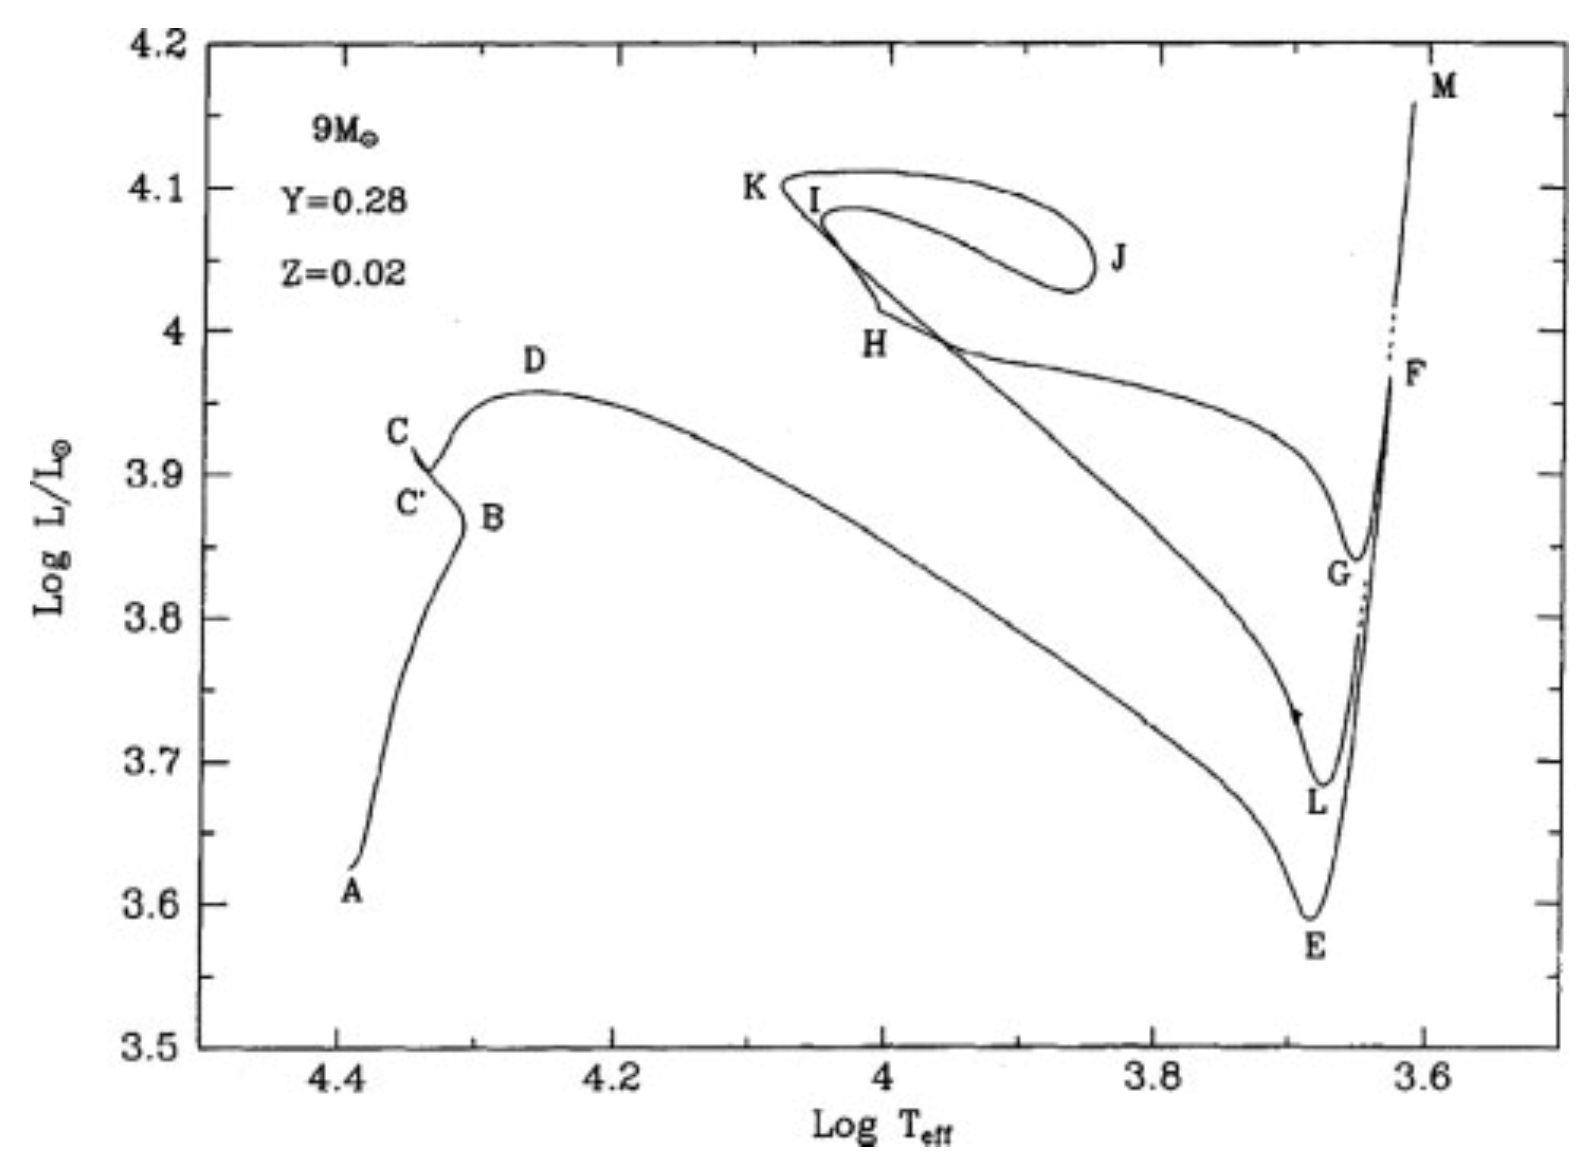
\includegraphics[width=10cm]{figures/HRD_9M.png}}
\end{figure}

{\noindent}Before disclosing what happens at points BDGHI and K (not mentioned in the previous list) it is necessary to introduce a few concepts in the language of stellar model makers. The \textbf{core} is the innermost part of the star, where nuclear reactions have greatly altered the original composition. By \textbf{envelope} one means the outer part of the star, over (most of) which nuclear burning is negligible and whose composition may still be close to the original one.

{\noindent}Next is the concept of \textbf{thermal equilibrium}. \textit{A star is said to be in thermal equilibrium (TE) when the total rate of nuclear energy generation ($L_N$) is almost perfectly equal to its surface luminosity ($L_S$).} TE means that the envelope is able to transfer outside and radiate into space quite precisely the same amount of energy which per unit time is produced by nuclear reactions in the core. If $L_S\simeq L_N$ the star is in TE and its evolution proceeds on a nuclear timescale. Conversely, if $L_S\neq L_N$ the star is out of TE, and its evolution proceeds on a thermal timescale, which usually is much shorter than the nuclear timescale. TE is often broken when the core runs out of fuel or when a new fuel is ignited. A dramatic example of breaking TE is the helium ignition in a degenerate core, called a \textbf{helium flash}. At flash peak $L_N\simeq 10^{10}\,{\rm L_\odot}$ while $L_S\simeq2000\,{\rm L_\odot}$ (and decreases!). The energy that does not escape the star is used to expand the helium core, hence relieving its degeneracy.

\begin{figure}[h]
    \floatbox[{\capbeside\thisfloatsetup{capbesideposition={right,top},capbesidewidth=4cm}}]{figure}[\FBwidth]
    {\caption{\footnotesize{The luminosity radiated from the star's surface as a function of the luminosity released by the stellar core and entering the envelope from its base, for the same track shown in Figure \ref{fig:hrd9}. Labels of relevant points along the sequence are the same as in Figure \ref{fig:hrd9}. Source: Renzini et al. (1992, Astrophys. J., 400, 280). Figure taken from Greggio \& Renzini (2011).}}
    \label{fig:lslb9}}
    {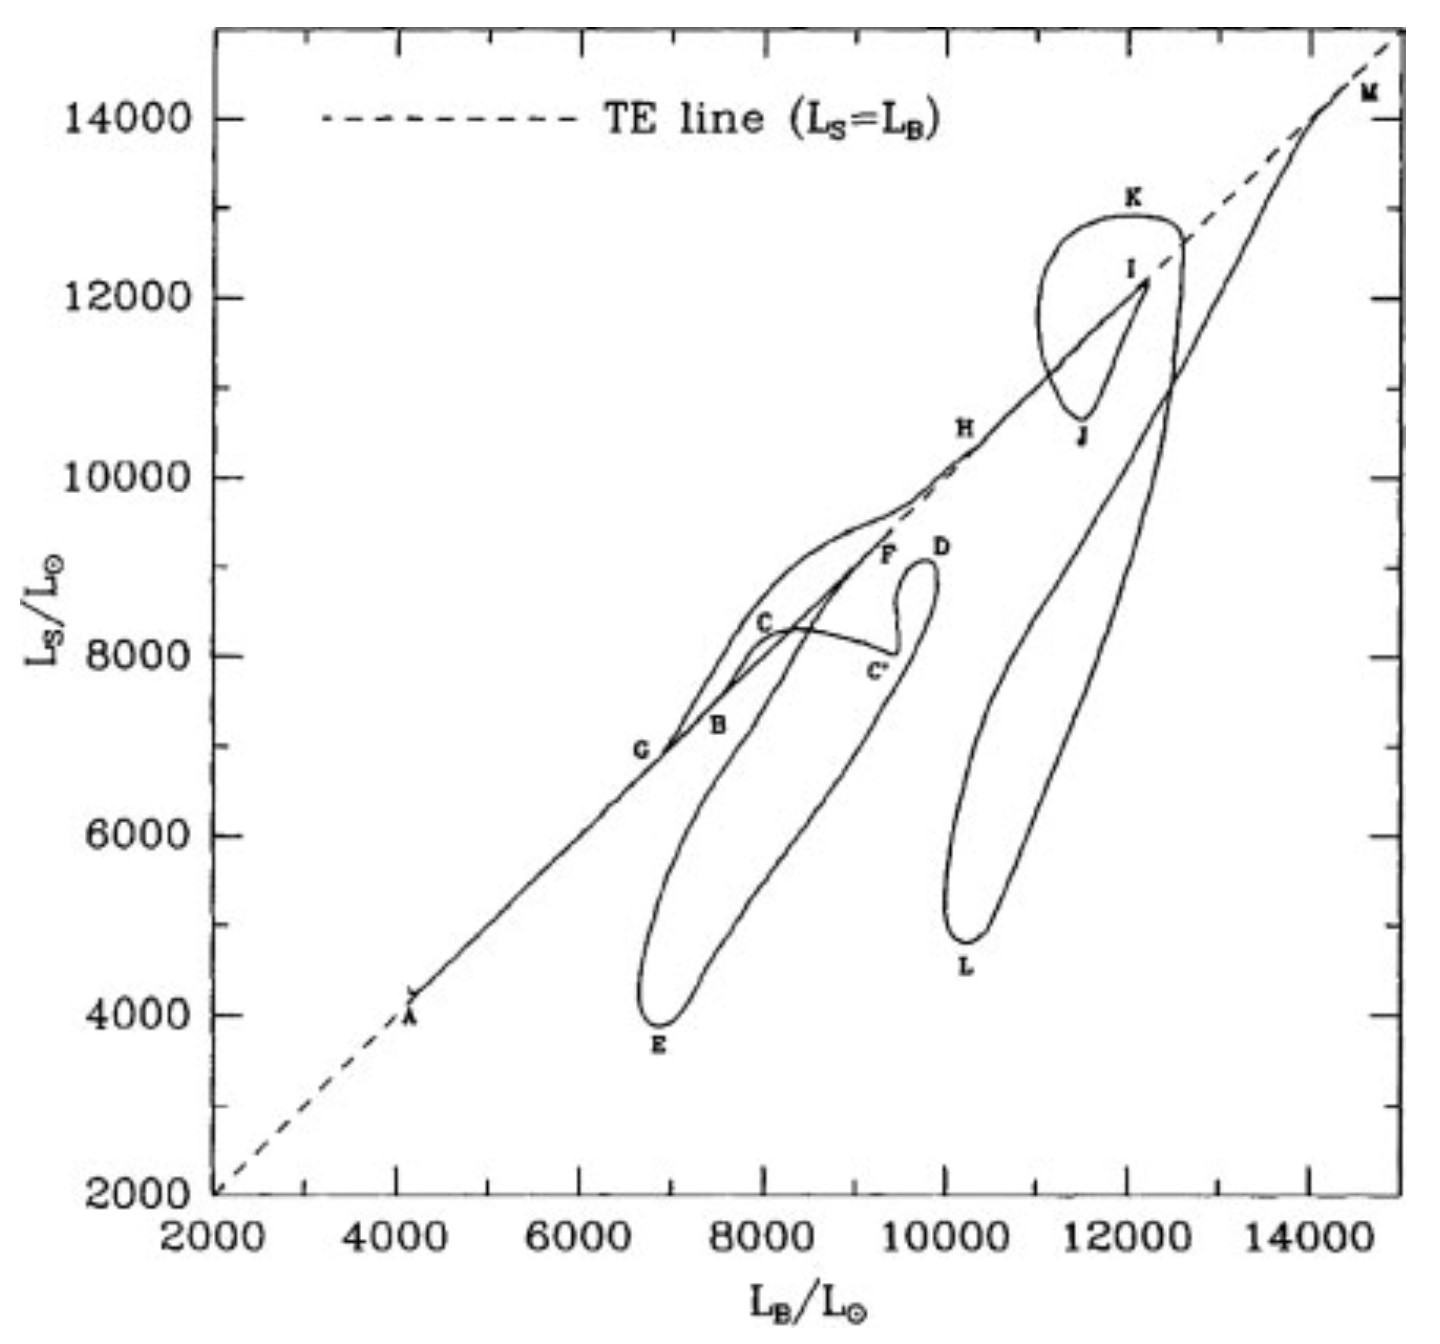
\includegraphics[width=10cm]{figures/LSLB_9M.png}}
\end{figure}

{\noindent}Evolutionary phases in TE and those out of TE can be easily identified by plotting $L_S$ versus $L_N$, or, equivalently, versus the luminosity impinging at the base of the envelope ($L_B$), as shown in Figure \ref{fig:lslb9} relative to the evolution of the same $9\,{\rm M_\odot}$ star model whose HRD is shown in Figure \ref{fig:hrd9}. Letter labels in this figure mark the same events as in Figure \ref{fig:hrd9}, so that one can identify those phases that are in TE and those which are out of it.

{\noindent}Thus, phase AB (which is most of the main sequence phase) proceeds in strict TE, but as hydrogen approaches exhaustion in the core, nuclear burning starts to fall short of keeping in pace with the rate at which energy is being radiated away, the star starts departing from TE and begins to contract (point B). At point B, as the core is running out of fuel the envelope starts losing more energy than it receives, and contracts until at point C hydrogen is effectively exhausted over the central regions, and nuclear energy generation quickly shifts to a shell surrounding a hydrogen-exhausted helium core. The quick readjustment from core to shell burning leaves the star at point C', somewhat out of TE, but then the structure tends to approach again TE, until at point D this tendency is reverted and a major excursion away from TE begins. In stars a little less massive than the one considered here, TE is actually well restored shortly after point C', and yet (as here at point D) TE is broken and stars undergo an extensive loop in the $L_S-L_B$ diagram, as shown in Figure \ref{fig:lslb9}. The journey across the HRD from point D to point E takes place on a thermal timescale, and the star expands to red giant dimensions. Clearly, a thermal instability erupts at point D. This is indeed a quite severe thermal instability, suffice to say from Figure \ref{fig:lslb9} that at the peak of the instability the core releases $\sim7000\,{\rm L_\odot}$ but the envelope radiates away only $\sim4000\,{\rm L_\odot}$, and $\sim3000\,{\rm L_\odot}$ are absorbed for its expansion.

{\noindent}The physical origin of this thermal instability is actually quite easy to understand. During phase C'D the luminosity provided by the hydrogen burning shell steadily increases as the shell moves out in the mass coordinate thanks to its own burning, and sits on a progressively more massive helium core. In response to the increasing luminosity impinging on its base ($L_B$) the envelope slowly expands. By expanding the envelope cools, and by cooling heavy metal ions begin to recombine. Besides being scattered by free electrons, photons now begin to be absorbed by such heavy ions via bound-bound and bound-free transitions: \textit{radiative opacity increases}. This opacity increase is the key factor that determines the onset of the thermal instability. At any point within the star the luminosity transmitted outwards by the radiation field is:

\begin{align*}
    L_r = 4\pi r^2 \frac{4acT^3}{3\kappa\rho} \frac{{\rm d}T}{{\rm d}r} = 4\pi r^2F_r ~ [{\rm erg\,s^{-1}}],
\end{align*}

{\noindent}where $r$ is the distance from the center, $T$ the temperature, $\rho$ the density, $\kappa$ the opacity, and $F_r$ the radiative energy flux. During phase C'D the envelope slowly expands, hence $r^2$ increases while the flux $F_r$ decreases, but their product still increases and the star is approaching TE. However, as this trend continues the increase in opacity accelerates and eventually the flux drops faster than $r^2$ increases, and their product $L_r$ starts to decrease. The decrease happens first near the stellar surface, and then (very quickly) through the whole envelope. At this point the envelope is transferring outwards and radiating away less energy than it receives from the stellar core, that is, $\Delta L=L_B-L_S>0$. But as the envelope expands more ions recombine, opacity increases further, the flux drops even more, the thermal imbalance $L_B-L_S$ increases and expansion accelerates: the stellar envelope is in a thermal runaway, as it becomes more and more unable to radiate away the energy it receives from the stellar interior.

{\noindent}At point E the surface luminosity starts to rise again, $L_B-L_S$ begins to drop, and TE is rapidly restored. What relieves the instability and saves the star from literally falling apart is convection. As the expanding envelope cools, and opacity increases, eventually the radiative gradient $\nabla_{\rm rad}$\footnote{Temperature gradients are defined as $\nabla T(\rho,T,X_i) = (\partial\log T/\partial\log P)$.} exceeds the adiabatic gradient $\nabla_{\rm ad}$, first near the photosphere, where hydrogen is only partly ionized, and then rapidly through the whole envelope. Thus, convection replaces radiative transfer in carrying out energy through the envelope, and the thermal instability is quenched since it was intimately related to the radiative mode of energy transfer. Most of the energy flux in the envelope being now carried by convective motions, the envelope ceases to absorb energy, and the surface luminosity LS starts to increase again: the star now ascends the Hayashi line, until at point F the helium burning reactions ignite in the core.

{\noindent}Following helium ignition, the helium core initiates a very slow expansion, which will last through a major fraction of the helium burning phase. This is because the helium burning core works like a breeder reactor during this stage, that is, it produces more new fuel than it burns. As \textbf{triple-$\mathbf{α}$} reactions produce fresh $^{12}$C, the $^{12}$C($\alpha,\gamma$)$^{16}$O reactions release an increasing amount of energy, and the inner core is forced to expand slightly. Such a modest expansion of the core is sufficient to cause a decrease of temperature and density in the surrounding hydrogen burning shell and the stellar luminosity correspondingly starts to decrease. The star now evolves along the \textbf{Hayashi line} from F to G, burning helium in the core and hydrogen in the shell, until thermal stability is broken again at point G. As the envelope contracts it heats up gradually, and in particular near its base, heavy ions start losing electrons. Hence opacity decreases along with the radiative gradient. As $\nabla_{\rm rad}$ drops below $\nabla_{\rm ad}$ a radiative region appears at the base of the envelope and grows outwards in mass. As this growth progresses the envelope becomes more and more transparent to radiation, until it starts radiating away more energy than it receives from the core: $L_B-L_S$ turns increasingly negative, the envelope starts deflating, but the more it contracts the more ``transparent'' it becomes, and the more energy it loses into space. The thermal instability bringing the star in its envelope deflation from point G to point H is precisely the reverse analog of the thermal instability that causes the runaway expansion from point D to point E. As envelope inflation can be ascribed to a runway recombination of heavy elements in the envelope, envelope deflation is due to a runway ionization of such heavy elements. A comparison of the three figures (Figures \ref{fig:hrd9}-\ref{fig:rvst}) helps in visualizing the onset of the thermal instability and of its results.

\begin{figure}[h]
    \floatbox[{\capbeside\thisfloatsetup{capbesideposition={right,top},capbesidewidth=4cm}}]{figure}[\FBwidth]
    {\caption{\footnotesize{The stellar radius as a function of time for the same track shown in Figure \ref{fig:hrd9}. Labels of relevant points along the sequence are the same as in Figure \ref{fig:hrd9}. Source: Renzini et al. (1992, Astrophys. J., 400, 280). Figure taken from Greggio \& Renzini (2011).}}
    \label{fig:rvst}}
    {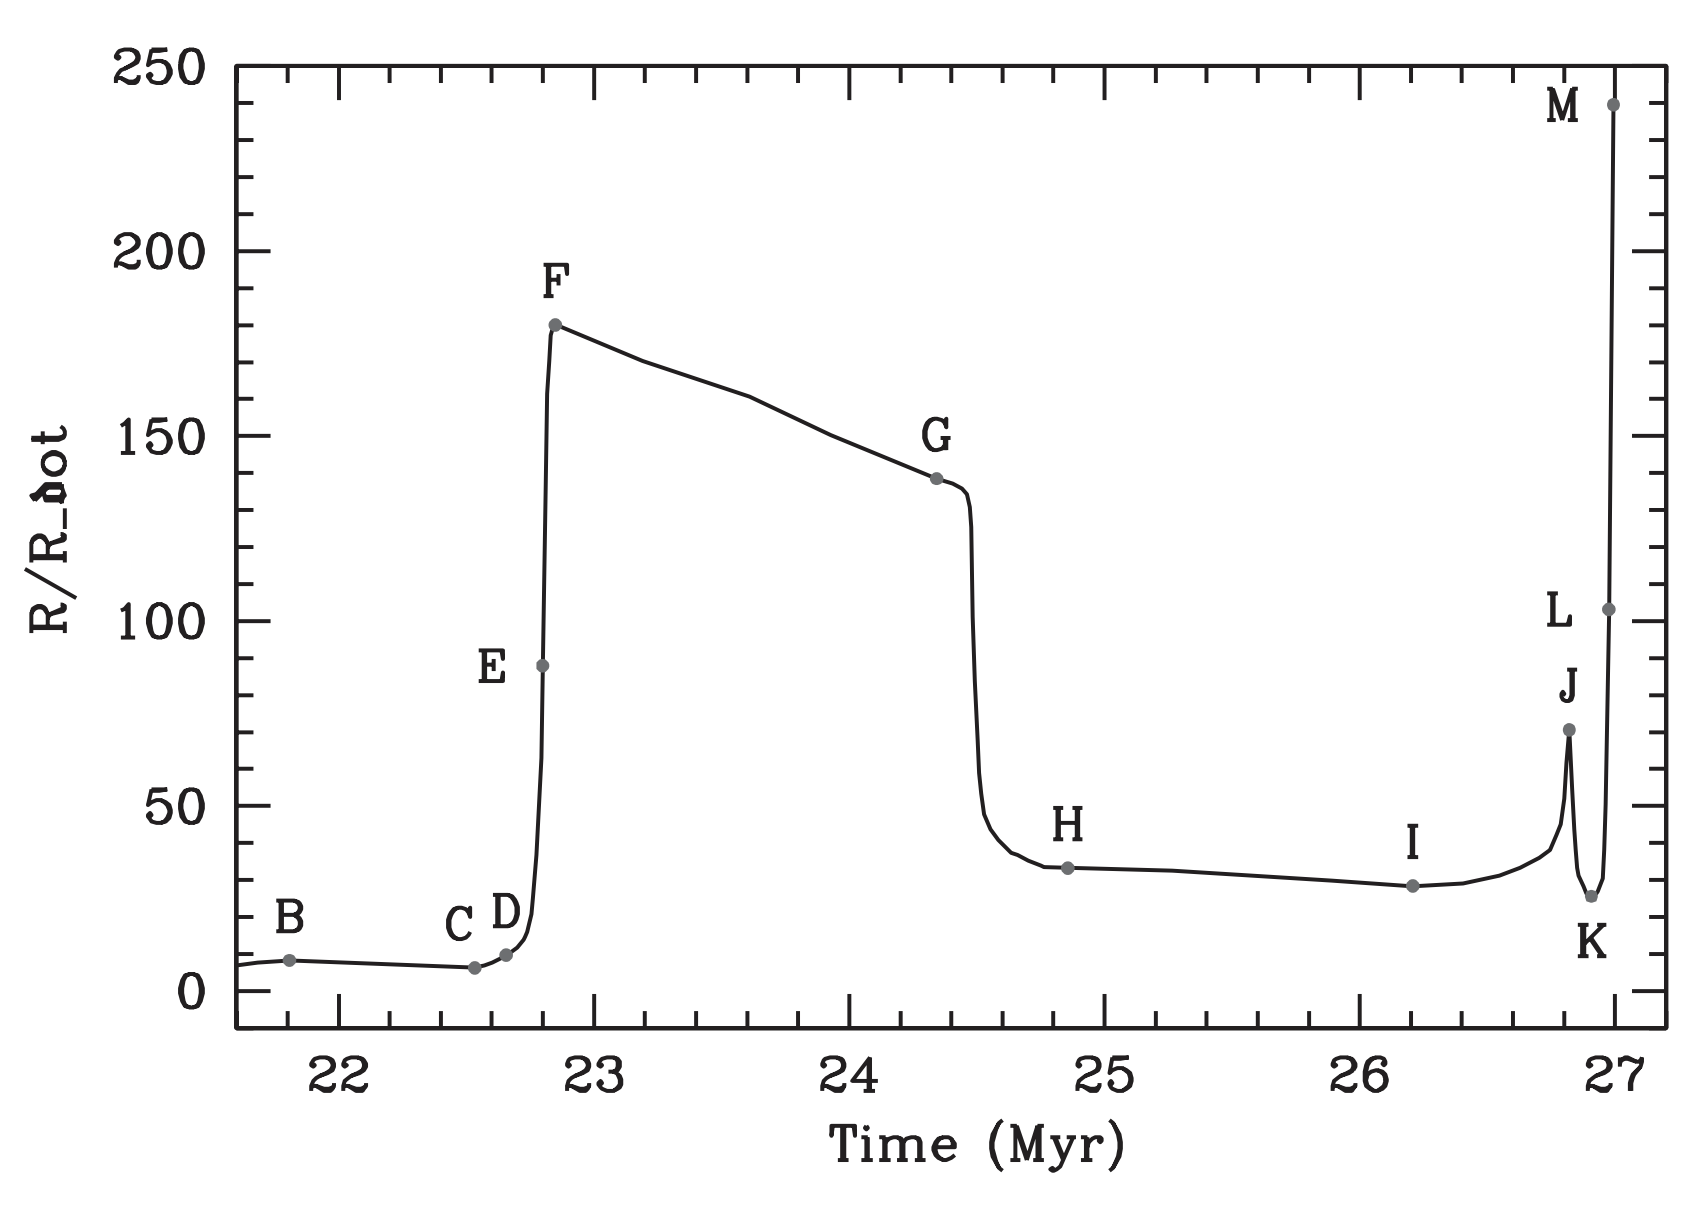
\includegraphics[width=10cm]{figures/RvsT.png}}
\end{figure}

{\noindent}Thus, in this star, the core helium burning phase in thermal equilibrium is spent in two distinct locations in the HRD: part on the Hayashi line as a red giant (F-G) and part as a blue giant (H-I) separated by a runaway contraction out of TE (G-H). This first blue loop (also called the \textbf{Cepheid blue loop}) continues after point I when TE is broken again. Here the envelope is slowly expanding in response to the slowly increasing luminosity from the core and shell burning, when the envelope turns unstable again due to the same physical process already described for the DE phase. 

{\noindent}However, the journey towards the Hayashi line is suddenly interrupted and inverted at point J, which marks the start of the so-called \textbf{second blue loop}. What happens at point J and after is a rather complex series of interconnected events: helium is exhausted in the core, the core contracts and helium burning rapidly shifts from the helium-exhausted CO core to a shell surrounding it; helium shell ignition is quite violent and causes expansion of the helium buffer above this shell: when the expansion front breaks through the hydrogen burning shell temperature and density in the shell drop; burning in the hydrogen shell (which was still providing most of the stellar luminosity) is effectively shut off completely causing a sudden drop of the luminosity impinging on the base of the envelope: $L_B$ drops below $L_S$ and the envelope stops expanding and contracts. In the meantime the strength of the helium burning shell steadily increases until it leads $L_B$ to exceed $L_S$ again, contraction stops and the star resumes at point K its runaway expansion that was temporarily stopped at J. The rest, from K to L to M is quite similar to the DEF phase, with convection replacing radiative transfer in the envelope and TE being rapidly restored, shortly before point M. Figure \ref{fig:rvst} clearly illustrates the dramatic effects of the envelope thermal instabilities on the overall structure of the star. Those phases which are in TE are nearly flat in this plot, that is, the stellar radius changes quite slowly with time. With one exception, those phases which are out of TE are instead nearly vertical, that is, the radius varies very rapidly during such runaway inflations or deflations. The exception is phase BC, which is only modestly out of TE, and contraction is relatively slow.

{\noindent}What happens past point M is still an open issue. A $9\,{\rm M_\odot}$ star lies between two domains: massive stars that eventually undergo core collapse and supernova explosion, and intermediate-mass stars, which shedding all their hydrogen-rich envelope die as a white dwarf. One believes that in a $9\,{\rm M_\odot}$ star carbon is ignited in the central core under only mildly degenerate conditions, and the star keeps ascending along the Hayashi line as a super asymptotic giant branch star experiencing a few thermal pulses in its deeper regions, where hydrogen and helium are still burning in two separate shells. Thus, if the envelope is completely lost in a wind the star leaves an ONeMg white dwarf. If instead mass loss is less severe then the core keeps growing in mass thanks to the active burning shells until electron captures in the core trigger a core collapse and we have a supernova explosion. Clearly the fate critically depends on the strength of the mass loss process.

{\noindent}\textbf{Evolution of a Solar-composition star:} Figure 1.4 shows stellar evolutionary tracks of solar composition, covering a wide range of initial masses, from a $0.8\,{\rm M_\odot}$ star, whose MS evolutionary lifetime is longer than one Hubble time, up to a $20\,{\rm M_\odot}$ model. The evolutionary tracks of stars with mass greater than $20\,{\rm M_\odot}$ are heavily affected by mass loss.

\begin{figure}[h]
    \floatbox[{\capbeside\thisfloatsetup{capbesideposition={right,top},capbesidewidth=4cm}}]{figure}[\FBwidth]
    {\caption{\footnotesize{Evolutionary tracks of solar composition star. The shaded area shows the location of low-mass ($0.55\leq M/M_\odot\leq2$) core helium burning models. Drawn using the YZVAR database (Bertelli, G. et al. 2008, Astron. Astrophys., 484, 815; 2009, Astron. Astrophys., 508, 355). Figure taken from Greggio \& Renzini (2011).}}
    \label{fig:hrdsolar}}
    {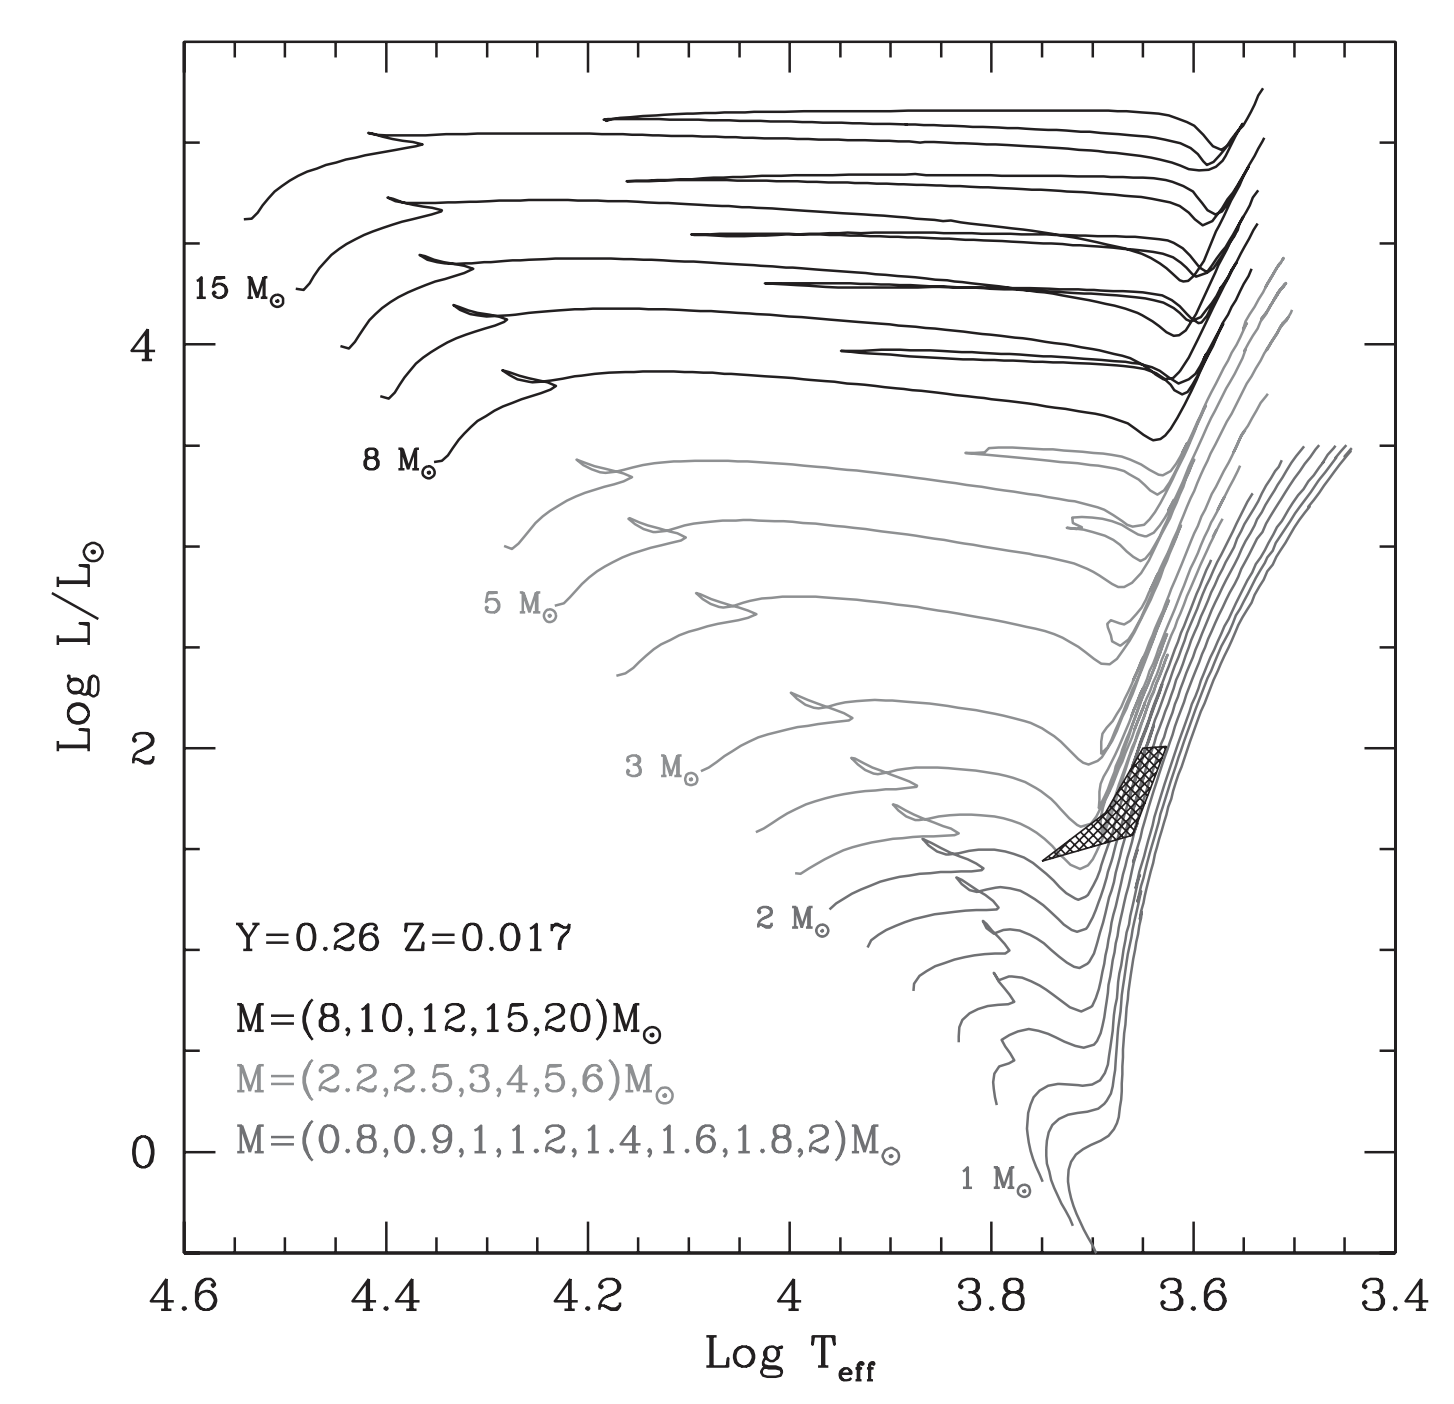
\includegraphics[width=10cm]{figures/HRD_Solar.png}}
\end{figure}

{\noindent}Different gray shades in Figure \ref{fig:hrdsolar} pertain to the different mass ranges as customarily distinguished in stellar evolution: low-mass stars, up to $\lesssim2.2\,{\rm M_\odot}$, intermediate-mass stars, up to $\lesssim8\,{\rm M_\odot}$, and high-mass stars. These ranges correspond to different physical behavior during the evolution of the stars, and the mass limits depend on chemical composition. Low-mass stars develop an \textbf{electron degenerate helium core} after their MS evolution; intermediate mass stars ignite helium under non-degenerate conditions, but develop a \textbf{CO degenerate core} after central helium burning; massive stars experience all successive nuclear burnings up to the production of an \textbf{iron core}.

{\noindent}During their MS evolution, stars with mass below $\sim1\,{\rm M_\odot}$ burn hydrogen through the \textbf{p-p chain}, whose reaction rate is not extremely sensitive to temperature, so that these stars possess a radiative core. As evolution proceeds hydrogen is progressively depleted in the inner core, more in the center than in the periphery, leading to a smooth hydrogen profile from a central minimum up to the initial abundance in the outer layers. On the HRD, the stellar track climbs to higher luminosities and temperatures until the central hydrogen is severely depleted; at this point the effective temperature starts decreasing, producing the turnoff (TO), that is, the maximum temperature point on the MS, which is easily recognizable on the CMD of globular clusters. Shortly after the TO, hydrogen is completely exhausted in the center and the hydrogen shell burning phase starts as a natural progression from the previous core hydrogen burning phase. During shell hydrogen burning, the track forms the subgiant branch (SGB), evolving at (almost) constant luminosity and decreasing temperature until the external convection penetrates deeply inside, and the star becomes almost fully convective at the base of the red giant branch (RGB).

{\noindent}The MS stars (with $M\gtrsim1\,{\rm M_\odot}$) have a convective core, since at least part of the hydrogen burning occurs through the CNO cycle, whose energy generation rate is extremely sensitive to temperature. Because of central mixing, the hydrogen profile is characterized by an inner plateau; as evolution proceeds, the extension of the convective core progressively decreases, leaving behind a gradient of hydrogen abundance. In stars with a convective core, the fuel depletion affects a sizable central region, which starts rapid contraction when approaching fuel exhaustion. This happens at the local minimum effective temperature point during the MS evolution of stars with $M>1\,{\rm M_\odot}$ (Figure \ref{fig:hrdsolar}), which signals the beginning of the overall contraction phase. The evolutionary behavior across this phase and the following runaway expansion has been already described in detail in the previous section.

{\noindent}As already mentioned, the helium core of low-mass stars is (electron) degenerate: this implies that central helium ignition is delayed because core contraction does not lead to an efficient increase of the central temperature. The (almost) fully convective star climbs along the RGB, while the hydrogen burning shell progresses outward, thereby increasing the mass of the helium core. When the core reaches a critical limit, a helium flash occurs off-center, since neutrino losses induce a temperature inversion in the innermost layers. This event in not catastrophic for the star because local expansion removes the degeneracy; instead, a sequence of flashes occurring at progressively inner locations totally remove the core degeneracy. During this phase, which lasts $1\,{\rm Myr}$, the star moves downward along the Hayashi line to settle on the core helium burning locus, either the red clump, or the horizontal branch (HB). The maximum luminosity reached on the RGB (RGB Tip, or TRGB) is a very important feature in the color-magnitude diagram (CMD) of stellar populations because it is virtually independent of mass, and then of evolutionary lifetime. This is because on the one hand the critical mass for helium ignition under degenerate conditions is almost constant ($0.5\,{\rm M_\odot}$), and on the other, along the RGB there exists a core mass-luminosity relation. The evolutionary lifetimes of low-mass stars range from $1\,{\rm Gyr}$ up to the Hubble time, as seen in Figure \ref{fig:hrdsolar}, and all of them experience the helium flash at almost the same luminosity; therefore, the CMD of a stellar population with stars older than $1\,{\rm Gyr}$ will show a prominent TRGB feature whose luminosity is known, thus allowing us to determine the distance of the stellar population. The TRGB luminosity depends slightly on metallicity, being higher for higher metal content. However, by a fortunate combination, the absolute magnitude in the I-band of the TRGB does not depend much on metallicity, for metal-poor populations. This is because the effective temperature at the TRGB also depends on metallicity: the higher $Z$, the cooler the TRGB stars, and the higher the bolometric correction (in absolute value). The trend with metallicity of the bolometric correction to the I-band largely compensates that of the tip luminosity, so that the I-band absolute magnitude of the TRGB ($M_{\rm I,TRGB}$) is almost independent of age and weakly dependent on metallicity of the parent stellar population. This makes $M_{\rm I,TRGB}$ a very effective distance indicator in galaxies.

{\noindent}The luminosity of core helium burning low-mass stars, being fixed by the mass of their hydrogen-exhausted core, is also largely independent of their total mass, thereby providing another distance indicator. However, evolution during the core helium burning phase spreads the red clump stars over $0.6$ magnitudes, as can be seen from the vertical size of the hatched region in Figure \ref{fig:hrdsolar}. In addition, the core mass at helium ignition is not a monotonic function of the total mass, and as the latter increases beyond the limit of the low-mass stars regime ($M_{\rm Hef}$), it decreases, reaches a minimum of about $0.326\,{\rm M_\odot}$, and then increases. As a result, stars with mass just above $M_{\rm Hef}$ start their core helium burning evolution at fainter luminosities, have the longest helium burning lifetimes, and cover a wider range of luminosities, compared to stars with $M<M_{\rm Hef}$. Therefore, the core helium burners of a composite stellar population with a sizable component at ages just below $1\,{\rm Gyr}$ are spread over a wide magnitude range, which limits the use of this feature for distance determinations.

{\noindent}The effective temperature of low mass core helium burning stars depends on the mass of their envelope, a dependence which is very pronounced when the envelope is thinner than for example $0.2\,{\rm M_\odot}$ for $Z\lesssim0.1\,{\rm Z_\odot}$. Below this threshold, the lower the envelope mass, the hotter the core helium burning stars. In a coeval and homogeneous stellar population the core helium burning stars all have virtually the same core mass and then luminosity; a spread of their envelope masses produces a feature on the HRD at about constant (bolometric) magnitude extending over a temperature range. The observational counterpart of this locus is the horizontal branch: a prominent feature in the HRD of globular clusters whose age is old enough to host core helium burning stars with low-mass envelopes. The existence of wide HBs in globular clusters was explained as due to a dispersion of mass lost during the RGB phase, but recently it became apparent that other effects are also at play. Evolutionary tracks during the core helium burning phase exhibit a wide variety of morphologies, depending on their mass, envelope mass, metallicity and helium abundance. At central helium exhaustion, a rapid core contraction leads to shell helium ignition; the model star expands and moves again towards the Hayashi line to start the asymptotic giant branch (AGB) evolutionary stage. However, if the envelope mass is small enough, the shell helium burning phase is entirely spent at high effective temperatures, as an AGB manqu\'e star. The hot HB stars and their AGB manqu\'e progeny are likely responsible for the UV emission from elliptical galaxies which host old stellar populations.

{\noindent}The evolution of intermediate and high-mass stars during the hydrogen and helium burning stages is very similar to what has already been described for the $9\,{\rm M_\odot}$ star. But, following helium exhaustion, intermediate-mass stars behave similarly to low-mass stars. We only notice here that for stars with mass in the vicinity of $M_{\rm Hef}$ the core helium burning phase is spent in a red clump, which becomes a wider and wider blue loop as the model mass grows. Thus, the core helium burning phase of intermediate-mass stars is spent part in the blue and part in the red. The very occurrence of the loop, its extension and the fraction of lifetime spent on each side of the loop, are sensitive to a number of parameters describing the input physics of the models, like metallicity, opacity, convection and others. Therefore, the blue-to-red ratio in stellar populations with stars in this mass range is difficult to interpret. The luminosity of intermediate mass core helium burners is instead a more robust prediction of the models, and can be effectively used as an age indicator of stellar populations.

\begin{table}[t]
    \centering
    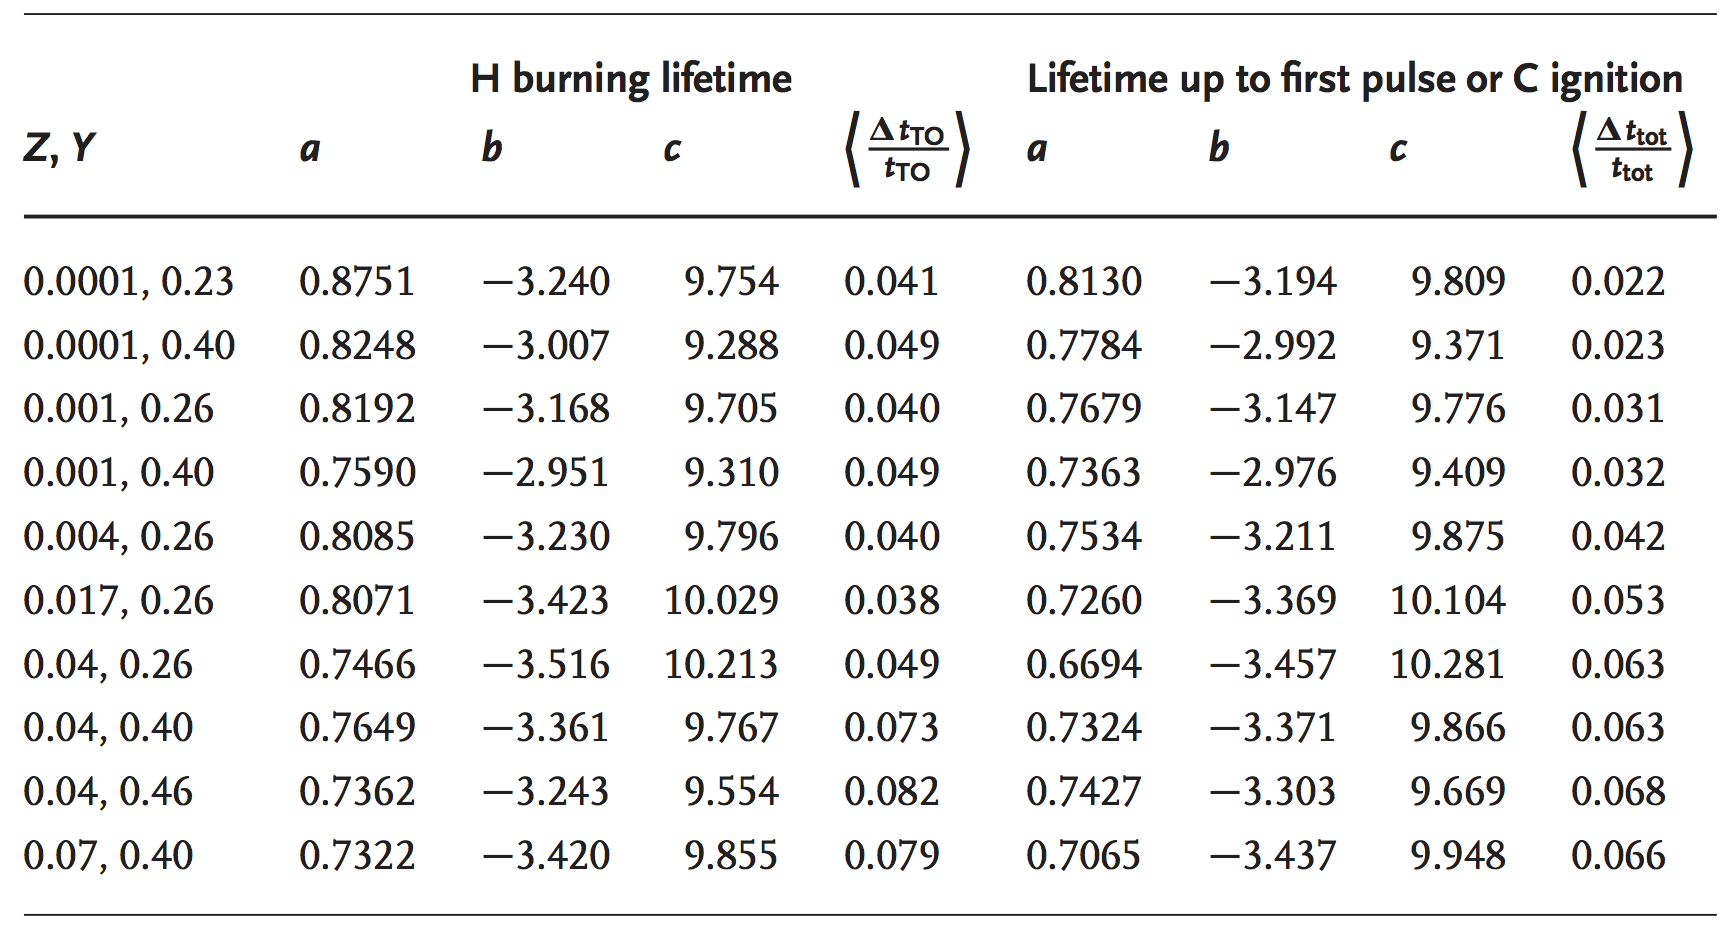
\includegraphics[width=10cm]{figures/HRD_Z_coeff.png}
    \caption{\footnotesize{Coefficients of $\log t$ for various chemical compositions, resulting from the least square fit of the hydrogen burning and the total lifetimes as a function of $M_0$. The fit covers the range $0.6\leq M_0/{\rm M_\odot} \leq20$; columns 5 and 9 report the average relative accuracy on the evolutionary lifetimes at the TO and at the first thermal pulse or central carbon ignition. The YZVAR database (Bertelli, G. et al. 2008, Astron. Astrophys., 484, 815; 2009, Astron. Astrophys., 508, 355) has been used to derive the coefficients. Table taken from Greggio \& Renzini (2011).}}
    \label{table:hrdz_coeff}
\end{table}

{\noindent}\textbf{Dependence on chemical composition:} The evolutionary tracks of given mass are very sensitive to the (initial) helium content ($Y$) and metallicity ($Z$), which control the energy generation rates and the opacity. We briefly illustrate some dependencies relevant to the interpretation of the HR diagram and of the spectral energy distribution of stellar populations.

{\noindent}At a given initial mass, evolutionary lifetimes become shorter as $Y$ increases, because stars with higher molecular weight are more compact, hotter, brighter, hence faster in consuming the hydrogen fuel, of which less is available. Instead, lifetimes become longer as $Z$ increases, because the hydrogen burning models get fainter due to the higher opacity, while the hydrogen fuel reservoir remains virtually unchanged. Table 1.2 lists the values of the coefficients of the following relation:

\begin{align*}
    \log t = a\log^2M_0 + b\log M_0 + c ~ [{\rm yr}],
\end{align*}

{\noindent}adopted to describe the evolutionary lifetimes (in years) as a function of initial mass (in ${\rm M_\odot}$). The parabolic fit over the whole considered mass range is a rather drastic approximation; nevertheless these analytic relations can be useful to estimate evolutionary lifetimes and their dependence on composition.

{\noindent}As mentioned previously, the values of mass defining the low, intermediate and high-mass range depend somewhat on chemical composition. For example $M_{\rm Hef}$ decreases with $Y$ increasing and with $Z$ decreasing. Therefore, an extended RGB on the HRD of a stellar population traces the presence of evolved stars with mass lower than $2.1\,{\rm M_\odot}$ for solar composition, or with mass lower than $1.5\,{\rm M_\odot}$ if $Z=0.001$, $Y=0.4$. However, evolutionary lifetimes at given mass also depend on composition, and, by and large, an extended and well populated RGB is developed in stellar populations older than $1\,{\rm Gyr}$ almost irrespective of chemical composition.

{\noindent}At fixed initial mass, zero age main sequence models are hotter and brighter for a higher helium content, and/or a lower metallicity. Indeed, the locus of the corresponding stars on the HRD (ZAMS) is used to infer the composition of the target stellar population, and is virtually the only way to estimate the helium content of these stars, if $Z$ is known from spectroscopy. The puzzling composition of multiple stellar populations in some galactic globular clusters has been derived from ZAMS fitting.

\begin{figure}[h]
    \floatbox[{\capbeside\thisfloatsetup{capbesideposition={right,top},capbesidewidth=4cm}}]{figure}[\FBwidth]
    {\caption{\footnotesize{a-c) Evolutionary tracks of intermediate-mass stars ($M/{\rm M_\odot}=3,4,5,6,7,8,10$) for different compositions, as labeled. In (a), the open circles mark start and the end of the core helium burning phase. Drawn using the BaSTI database (Pietrinferni, A. et al. 2004, Astrophys. J., 612, 168). the Figure taken from Greggio \& Renzini (2011).}}
    \label{fig:hrdz_int}}
    {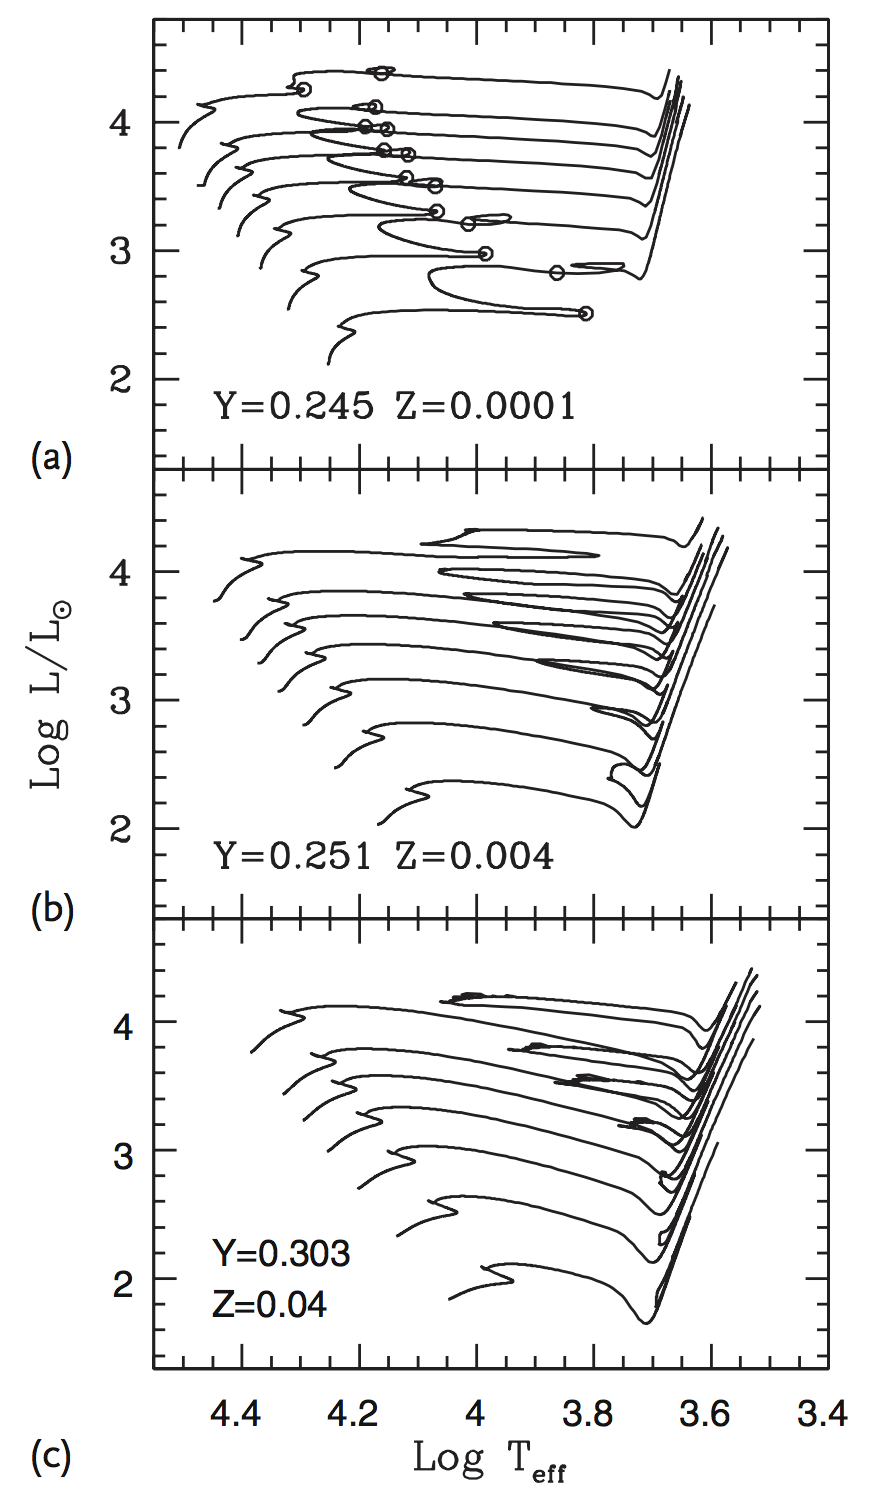
\includegraphics[width=8cm]{figures/HRD_Z_int.png}}
\end{figure}

{\noindent}Figure \ref{fig:hrdz_int} shows some evolutionary tracks of intermediate-mass stars for three different initial compositions. The described trend of the ZAMS with metal content is readily visible, together with some other properties already mentioned: at very low metallicity (Figure \ref{fig:hrdz_int}a) the entire core helium burning phase occurs in the blue part of the HRD, and the thermal runaway in the envelope which brings the model star to the Hayashi track is delayed to the very latest stages. As metallicity increases, the luminosity decrease associated with the thermal runaway gets more and more pronounced: this reflects the progressively higher opacity, and then radiative energy trapping in the envelope. At the same time, at higher metallicity it is more difficult to produce extended blue loops: the $3$ and $4\,{\rm M_\odot}$ tracks at $Z\sim2\,{\rm Z_\odot}$ do not present a blue loop at all, and the loop of the $5\,{\rm M_\odot}$ track is just alluded to. The models in Figure \ref{fig:hrdz_int} are computed adopting classical recipes for the input physics, and even slight modifications of the assumptions lead to dramatic variations of the tracks shape. For example, intermediate-mass models with $Z=0.04$, $Y=0.40$ which adopt a modest overshooting from the convective core lack the loops completely, and the core helium burning phase is totally spent close to the Hayashi line.

{\noindent}Figure \ref{fig:hrdz_low} illustrates the effect of chemical composition on core helium burners of low-mass. The gray tracks in Figure \ref{fig:hrdz_low}a show that at solar composition this evolutionary phase is completely spent in the red, even for masses as low as $0.55\,{\rm M_\odot}$. Conversely, at low metallicity (black lines), low-mass core helium burners are blue, opening the possibility of producing extended HBs in old stellar populations. The tracks in Figure 1.6b show the effect of enhancing the helium abundance: at high metallicity the core helium burning phase is completely spent close to the Hayashi line for a solar helium abundance, but if the helium abundance is high, a blueward excursion occurs during the core helium burning phase which is very wide for low-mass stars. Therefore the production of blue HB stars in old stellar populations can be achieved either assuming heavy mass loss on the RGB, or a high helium content, or both. Actually, the existence of multiple stellar populations with different helium content in NGC 2808 has been first suggested on the basis of its HB stars distribution, and confirmed later from the multiple MSs. Mass loss and helium abundance have indeed an important impact on the HRD of stellar populations, as well as on their spectral energy distribution, since stars in the core helium burning phase provide an important contribution to the total light.

\begin{figure}[t]
    \centering
    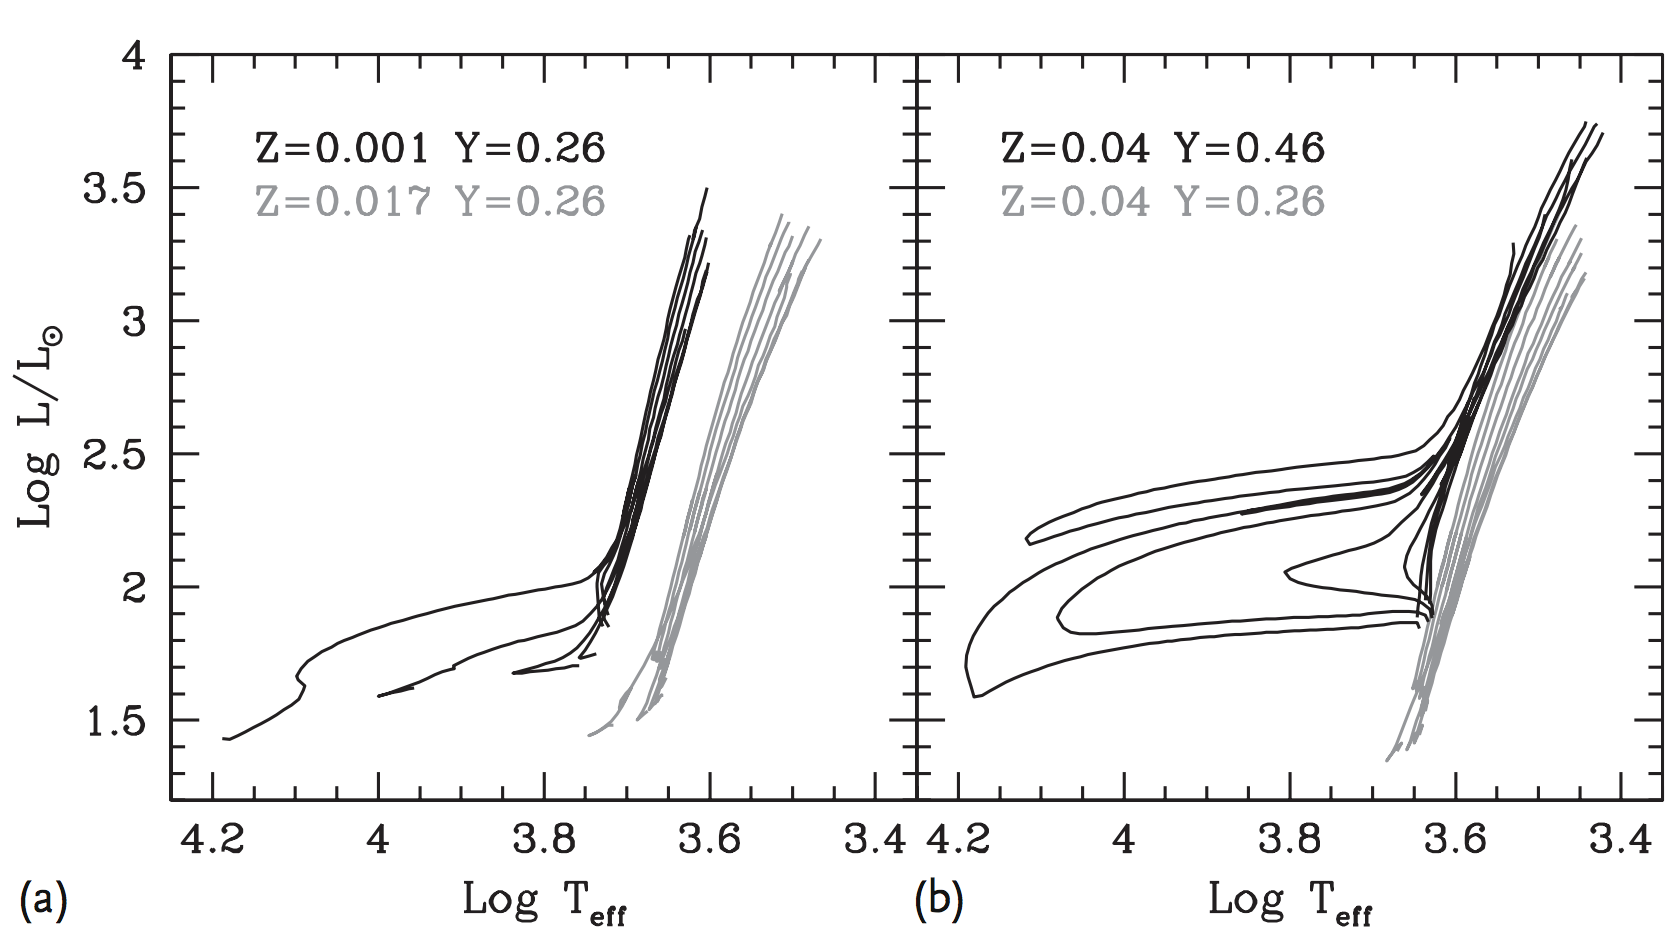
\includegraphics[width=14cm]{figures/HRD_Z_low.png}
    \caption{\footnotesize{(a,b) Evolutionary tracks of low-mass stars during the core helium burning and early AGB phases. The chemical composition is labeled. Initial model masses are $M/{\rm M_\odot}=0.55,0.6,0.65,0.7,1,1.2,1.4,1.6$ except for the ($Z=0.04,Y=0.46$) set, for which the $1.6\,{\rm M_\odot}$ track ignites helium under non-degenerate conditions. Drawn using the YZVAR database (Bertelli, G. et al. 2008, Astron. Astrophys., 484, 815; 2009, Astron. Astrophys., 508, 355). Figure taken from Greggio \& Renzini (2011).}}
    \label{fig:hrdz_low}
\end{figure}

\begin{itemize}
    \item How does metallicity affect this diagram?
    \item Elaborate on the life sequence of low-mass stars.
    \item Elaborate on the life sequence of high-mass stars.
    \item Which direction does radius increase?
    \item What's the functional form for how radius increases as a function of temperature and luminosity?
    \item Why can you use the tip of the red giant branch for distance determination?
    \item How can you use the H-R diagram to determine ages? Which of the two techniques is more accurate?
\end{itemize}

% --------------------------------------------------------------
%               2. 
% --------------------------------------------------------------

\newpage
\subsection{Question 2}

Sketch a plot of radius versus mass for various ``cold'' objects made of normal matter, including planets, brown dwarfs and white dwarfs. Explain the mass-size relationship for rocky and
gaseous objects. Why is there an upper mass limit?

\subsubsection{Short answer}

Answer.

\subsubsection{Additional context}

Additional context.

\subsubsection{Follow-up Questions}

\begin{itemize}
    \item How do you calculate the Chandrasekhar mass limit?
    \item Why is Saturn smaller than Jupiter? Or, why do we see a range of radii in extrasolar planets (e.g., hot Jupiters)?
\end{itemize}

% --------------------------------------------------------------
%               3. 
% --------------------------------------------------------------

\newpage
\subsection{Question 3}

Describe the physical conditions that lead to the formation of absorption lines in stars' spectra. What leads to emission lines?

\subsubsection{Short answer}

Answer.

\subsubsection{Additional context}

If an absorber $X$ is in a level $\ell$ and there is radiation present with photons having an energy equal to $E_u-E_\ell$, where $E_\ell$ and $E_u$ are the energies of levels $\ell$ (for ``lower'') and $u$ (for ``upper''), the absorber can absorb a photon and undergo an upward transition:

\begin{align*}
    \mathbf{absorption:} ~~~ X_\ell+h\nu\rightarrow X_u, ~~~ h\nu=E_u-E_\ell.
\end{align*}

{\noindent}Suppose that we have number density $n_\ell$ of absorbers $X$ in level $\ell$. The rate per volume at which the absorbers absorb photons will obviously be proportional to both the density of photons of the appropriate energy and the number density $n_\ell$, so we can write the rate of change of $n_\ell$ due to photo-absorption by level $\ell$ as

\begin{align*}
    \left(\frac{{\rm d}n_u}{{\rm d}t}\right)_{\ell\rightarrow u} = -\left(\frac{{\rm d}n_\ell}{{\rm d}t}\right)_{\ell\rightarrow u} = n_\ell B_{\ell u}u_\nu, ~~~ \nu=\frac{E_u-E_\ell}{h},
\end{align*}

{\noindent}where $u_\nu$ is the \textbf{radiation energy density per unit frequency}, and the proportionality constant $B_{\ell u}$ is the \textbf{Einstein B coefficient} for the transition $\ell\rightarrow u$.

{\noindent}An absorber $X$ in an excited level $u$ can decay to a lower level $\ell$ with emission of a photon. There are two ways this can happen:

\begin{align*}
    \mathbf{spontaneous~emission:} X_u&\rightarrow X_\ell+h\nu, ~~~ \nu=(E_u-E_\ell)/h, \\
    \mathbf{stimulated~emission:} X_u+h\nu&\rightarrow X_\ell+2h\nu, ~~~ \nu=(E_u-E_\ell)/h.
\end{align*}

{\noindent}\textbf{Spontaneous emission} is a random process, independent of the presence of a radiation field, with a probability per unit time $A_{u\ell}$ -- the \textbf{Einstein A coefficient}.

{\noindent}\textbf{Stimulated emission} occurs if photons of the identical frequency, polarization, and direction of propagation are already present, and the rate of stimulated emission is proportional to the density of these photons. Thus the total rate of depopulation of level $u$ due to emission of photons can be written

\begin{align*}
    \left(\frac{{\rm d}n_\ell}{{\rm d}t}\right)_{u\rightarrow\ell} = -\left(\frac{{\rm d}n_u}{{\rm d}t}\right)_{u\rightarrow\ell} = n_u(A_{u\ell}+B_{u\ell}u_\nu), ~~~ \nu=\frac{E_u-E_\ell}{h},
\end{align*}

{\noindent}where the coefficient $B_{u\ell}$ is the \textbf{Einstein B coefficient} for the downward transition $u\rightarrow\ell$. Thus we now have three coefficients characterizing radiative transitions between levels $u$ and $\ell$: $A_{u\ell}$, $B_{u\ell}$ and $B_{\ell u}$. We will now see that they are not independent of one another.

{\noindent}In TE, the radiation field becomes the ``blackbody'' radiation field, with intensity given by the \textbf{blackbody spectrum}

\begin{align*}
    B_\nu(T) = \frac{2h\nu^2}{c^2} \frac{1}{\exp(h\nu/k_BT) - 1} ~ [{\rm erg\,s^{-1}\,cm^{-2}\,Hz^{-1}\,sr^{-1}}],
\end{align*}

{\noindent}with specific energy density

\begin{align*}
    (u_\nu)_{\rm LTE} = \frac{4\pi}{c}B_\nu(T) = \frac{8\pi h\nu^3}{c^3}\frac{1}{e^{h\nu/k_BT}-1} ~ [{\rm erg\,s^{-2}\,cm^{-1}\,Hz^{-1}\,sr^{-1}}].
\end{align*}

{\noindent}If we place absorbers $X$ into a blackbody radiation field, then the net rate of change of level $u$ is

\begin{align*}
    \frac{{\rm d}n_u}{{\rm d}t} &= \left(\frac{{\rm d}n_u}{{\rm d}t}\right)_{\ell\rightarrow u} + \left(\frac{{\rm d}n_u}{{\rm d}t}\right)_{u\rightarrow\ell} \\
    &= n_\ell B_{\ell u}\frac{8\pi h\nu^3}{c^3} \frac{1}{\exp(h\nu/k_BT) - 1} - n_u \left(A_{u\ell}+B_{u\ell}\frac{8\pi h\nu^3}{c^3} \frac{1}{\exp(h\nu/k_BT) - 1}\right).
\end{align*}

{\noindent}If the absorbers are allowed to come to equilibrium with the radiation field, levels $\ell$ and $u$ must be populated according to $n_u/n_\ell = (g_u/g_\ell)e^{(E_\ell−E_u)/k_BT}$, with ${\rm d}n_u/{\rm d}t = 0$. From the equation above, it is easy to show that $B_{u\ell}$ and $B_{\ell u}$ must be related to $A_{u\ell}$ by

\begin{align*}
    B_{u\ell} &= \frac{c^3}{8\pi h\nu^3}A_{u\ell} ~ [{\rm s^{-1}}], \\
    B_{\ell u} &= \frac{g_u}{g_\ell}B_{u\ell} = \frac{g_u}{g_\ell}\frac{c^3}{8\pi h\nu^3} A_{u\ell} ~ [{\rm s^{-1}}].
\end{align*}

{\noindent}Thus the strength of stimulated emission ($B_{u\ell}$) and absorption ($B_{\ell u}$) are both determined by $A_{u\ell}$ and the ratio $g_u/g_\ell$.

{\noindent}Rather than discussing absorption and stimulated emission in terms of the radiation energy density $u_\nu$, it is helpful to characterize the intensity of the radiation field by a dimensionless quantity, the photon occupation number $n_\gamma$:

\begin{align*}
    n_\gamma &\equiv \frac{c^2}{2h\nu^3} I_\nu ~ [{\rm dimensionless}], \\
    \bar{n}_\gamma &\equiv \frac{c^2}{2h\nu^3} \bar{I}_\nu = \frac{c^3}{8\pi h\nu^3} u_\nu ~ [{\rm dimensionless}],
\end{align*}

{\noindent}where the bar denotes averaging over directions. With this definition of $n_\gamma$, we can rewrite equations for $({\rm d}n_u/{\rm d}t)_{\ell\rightarrow u}$ and $({\rm d}n_\ell/{\rm d}t)_{u\rightarrow\ell}$ as simply

\begin{align*}
    \left(\frac{{\rm d}n_\ell}{{\rm d}t}\right)_{u\rightarrow\ell} &= n_uA_{u\ell}(1+\bar{n}_\gamma),\\
    \left(\frac{{\rm d}n_u}{{\rm d}t}\right)_{\ell\rightarrow u} &= n_\ell \frac{g_u}{g_\ell}A_{u\ell}\bar{n}_\gamma.
\end{align*}

{\noindent}If the radiation field depends on frequency in the vicinity of the transition frequency $\nu_{u\ell}$, then $n_\gamma$ needs to be averaged over the emission and absorption profiles in the above two equations.

{\noindent}From the first of the above two equations, we immediately see that the photon occupation number $n_\gamma$ determines the relative importance of stimulated and spontaneous emission: stimulated emission is unimportant when $\bar{n}_\gamma\ll1$, but should otherwise be included in analyses of level excitation.

{\noindent}\textbf{Absorption cross section:} Having determined the rate at which photons are absorbed by an absorber exposed to electromagnetic radiation, it is useful to recast this in terms of an absorption cross section. The photon density per unit frequency is just $u_\nu/h\nu$. Let $\sigma_{\ell u}(\nu)$ be the cross section for absorption of photons of frequency $\nu$ with resulting $\ell\rightarrow u$ transition. The absorption rate is then

\begin{align*}
    \left(\frac{{\rm d}n_u}{{\rm d}t}\right)_{\ell\rightarrow u}= n_\ell \int \sigma_{\ell u}(\nu)c \frac{u_\nu}{h\nu}{\rm d}\nu \approx n_\ell u_\nu \frac{c}{h\nu} \int \sigma_{\ell u}(\nu){\rm d}\nu ~ [{\rm s^{-1}}],
\end{align*}

{\noindent}where we have assumed that $u_\nu$ (and $h\nu$) do not vary appreciably over the line profile of $\sigma_{u\ell}$. Thus

\begin{align*}
    B_{\ell u} = \frac{c}{h\nu} \int \sigma_{\ell u}(\nu){\rm d}\nu ~ [{\rm s^{-1}}],
\end{align*}

{\noindent}and, using our equation that relates $B_{\ell u}$ to $A_{u\ell}$, we obtain the integral over the absorption cross section:

\begin{align*}
    \int \sigma_{\ell u}(\nu){\rm d}\nu = \frac{g_u}{g_\ell} \frac{c^2}{8\pi\nu_{\ell u}^2}A_{u\ell} ~ [{\rm Hz\,cm^2}].
\end{align*}

{\noindent}Thus we may relate the monochromatic absorption cross section $\sigma_{\ell u}(\nu)$ to a normalized line profile $\phi_\nu$:

\begin{align*}
    \sigma_{\ell u}(\nu) = \frac{g_u}{g_\ell} \frac{c^2}{8\pi\nu_{\ell u}^2}A_{u\ell} \phi_\nu ~ [{\rm cm^2}], ~~~ \int\phi_\nu{\rm d}\nu =1.
\end{align*}

{\noindent}\textbf{Intrinsic line profile:} The intrinsic line profile is characterized by a normalized profile function $\phi_\nu^{\rm intr}$:

\begin{align*}
    \sigma_\nu^{\rm intr} = \frac{\pi e^2}{m_ec^2}f_{\ell u} \phi_\nu^{\rm intr} ~ [{\rm cm^2}], ~~~ \int\phi_\nu^{\rm intr}{\rm d}\nu =1.
\end{align*}

{\noindent}The intrinsic line profile of an absorption line is normally described by the \textbf{Lorentz line profile} function:

\begin{align*}
    \phi_\nu^{\rm intr} = \frac{4\gamma_{u\ell}}{16\pi^2(\nu-\nu_{u\ell})^2+\gamma_{u\ell}^2} ~ [{\rm erg\,s^{-1}\,cm^{-2}\,sr^{-1}}],
\end{align*}

{\noindent}where $\nu_{u\ell} \equiv (E_u-E_\ell)/h$. The Lorentz profile provides an accurate (but not exact)\footnote{The line profile is more accurately given by the \textbf{Kramers-Heisenberg formula}; Lee (2003) discusses application of this formula to the Lyman $\alpha$ line.} approximation to the actual line profile. The Lorentz line profile has a \textbf{full width at half maximum} (FWHM) of

\begin{align*}
    (\Delta\nu)_{\rm FWHM}^{\rm intr} = \frac{\gamma_{u\ell}}{2\pi} ~ [{\rm Hz}].
\end{align*}

{\noindent}The intrinsic width of the absorption line reflects the uncertainty in the energies of levels $u$ and $\ell$ due to the finite lifetimes of these levels\footnote{The \textbf{Heisenberg uncertainty principle} $\Delta E\Delta t\geq\hbar$ implies that an energy level $u$ has a width $\Delta E_u\approx\hbar/\tau_u$, where $\tau_u$ is the level lifetime.} against transitions to all other levels, including both radiative and collisional transitions. If the primary process for depopulating levels $u$ and $\ell$ is spontaneous decay (as is often the case in the ISM), then

\begin{align*}
    \gamma_{u\ell} \equiv \gamma_{\ell u} = \sum_{E_j<E_u}A_{uj} + \sum_{E_j<E_\ell}A_{\ell j}.
\end{align*}

{\noindent}In the case of a \textbf{resonance line}, where $\ell$ is the ground state, the second sum vanishes.

{\noindent}\textbf{Doppler broadening; The voigt line profile:} Atoms and ions are generally in motion, and the velocity distribution is often approximated by a Gaussian, this being of course the correct form if the velocities are entirely due to thermal motions:

\begin{align*}
    p_v = \frac{1}{\sqrt{2\pi}}\frac{1}{\sigma_v} e^{-(v-v_0)^2/2\sigma_v^2} = \frac{1}{\sqrt{\pi}}\frac{1}{b} e^{-(v-v_0)^2/b^2},
\end{align*}

{\noindent}where $p_v{\rm d}v$ is the probability of the velocity along the line of sight being in the interval $[v,v+{\rm d}v]$, $\sigma_v$ is the one-dimensional velocity dispersion, and $b$ is the the \textbf{broadening parameter}, $b\equiv\sqrt{2}\sigma_v$.

{\noindent}The width of the velocity distribution is also sometimes specified in terms of the FWHM; for a Gaussian distribution of velocities, this is just

\begin{align*}
    (\Delta v)_{\rm FWHM} = \sqrt{8\ln2}\sigma_v = 2\sqrt{\ln2}b ~ [{\rm m\,s^{-1}}].
\end{align*}

{\noindent}If the velocity dispersion is entirely due to thermal motion with kinetic temperature $T=10^4T_4\,{\rm K}$, then

\begin{align*}
    \sigma_v &= \left(\frac{k_BT}{M}\right)^{1/2} = 9.12\left(\frac{T_4}{M/{\rm amu}}\right)^{1/2} ~ [{\rm km\,s^{-1}}] \\
    b &= \left(\frac{2k_BT}{M}\right)^{1/2} = 12.90\left(\frac{T_4}{M/{\rm amu}}\right)^{1/2} ~ [{\rm km\,s^{-1}}] \\
    (\Delta v)_{\rm FWHM}^{\rm therm} &= \left[\frac{(8\ln2)k_BT}{M}\right]^{1/2} = 21.47\left(\frac{T_4}{M/{\rm amu}}\right)^{1/2} ~ [{\rm km\,s^{-1}}].
\end{align*}

{\noindent}The intrinsic absorption line profile $\phi_\nu^{\rm intr}$ must be convolved with the velocity distribution of the absorbers to obtain the line profile

\begin{align*}
    \phi_\nu = \int p_v(v) \frac{4\gamma_{u\ell}}{16\pi^2[\nu-(1-v/c)\nu_{u\ell}]^2 + \gamma_{u\ell}^2}{\rm d}v ~ [{\rm erg\,s^{-1}\,cm^{-2}\,sr^{-1}}],
\end{align*}

{\noindent}where $p_v{\rm d}v$ is the probability of the absorber having radial velocity in the interval $[v,v+{\rm d}v]$. If the absorbers have a \textbf{Maxwellian} (i.e., Gaussian) one-dimensional velocity distribution $p_v$, then the absorption line will have a so-called \textbf{Voigt line profile}:

\begin{align*}
    \phi_\nu^{\rm Voigt} \equiv \frac{1}{\sqrt{2\pi}} \int \frac{e^{-v^2/2\sigma_v^2}}{\sigma_v} p_v(v) \frac{4\gamma_{u\ell}}{16\pi^2[\nu-(1-v/c)\nu_{u\ell}]^2 + \gamma_{u\ell}^2}{\rm d}v ~ [{\rm erg\,s^{-1}\,cm^{-2}\,sr^{-1}}].
\end{align*}

{\noindent}Unfortunately, the Voigt line profile cannot be obtained analytically except for limiting cases.5 However, if, as is generally the case, the one-dimensional velocity dispersion $\sigma_v\gg (\Delta v)_{\rm FWHM}^{\rm intr}$, the central core of the line profile is well-approximated by treating the intrinsic line profile as a $\delta$-function, so that the central core of the line has a Maxwellian profile:

\begin{align*}
    \phi_\nu \approx \frac{1}{\pi} \frac{1}{\nu_{u\ell}}\frac{c}{b} e^{-v^2/b^2} ~ [{\rm erg\,s^{-1}\,cm^{-2}\,sr^{-1}}], ~~~ b\equiv\sqrt{2}\sigma_v.
\end{align*}

{\noindent}\textbf{Selection rules for radiative transitions:} Some energy levels are connected by strong radiative transitions; in other cases, radiative transitions between the levels may be extremely slow. The strong transitions always satisfy what are referred to as the \textbf{selection rules for electric dipole transitions}. Here, we summarize the selection rules for the strong electric dipole transitions, and we also give the selection rules for \textbf{inter-system} and \textbf{forbidden transitions} that do not satisfy the electric dipole selection rules but nevertheless are strong enough to be astrophysically important. We will use the ion NII as an example; the first nine energy levels of NII are shown in Figure \ref{fig:NIIlevels}.

\begin{figure}[t]
    \centering
    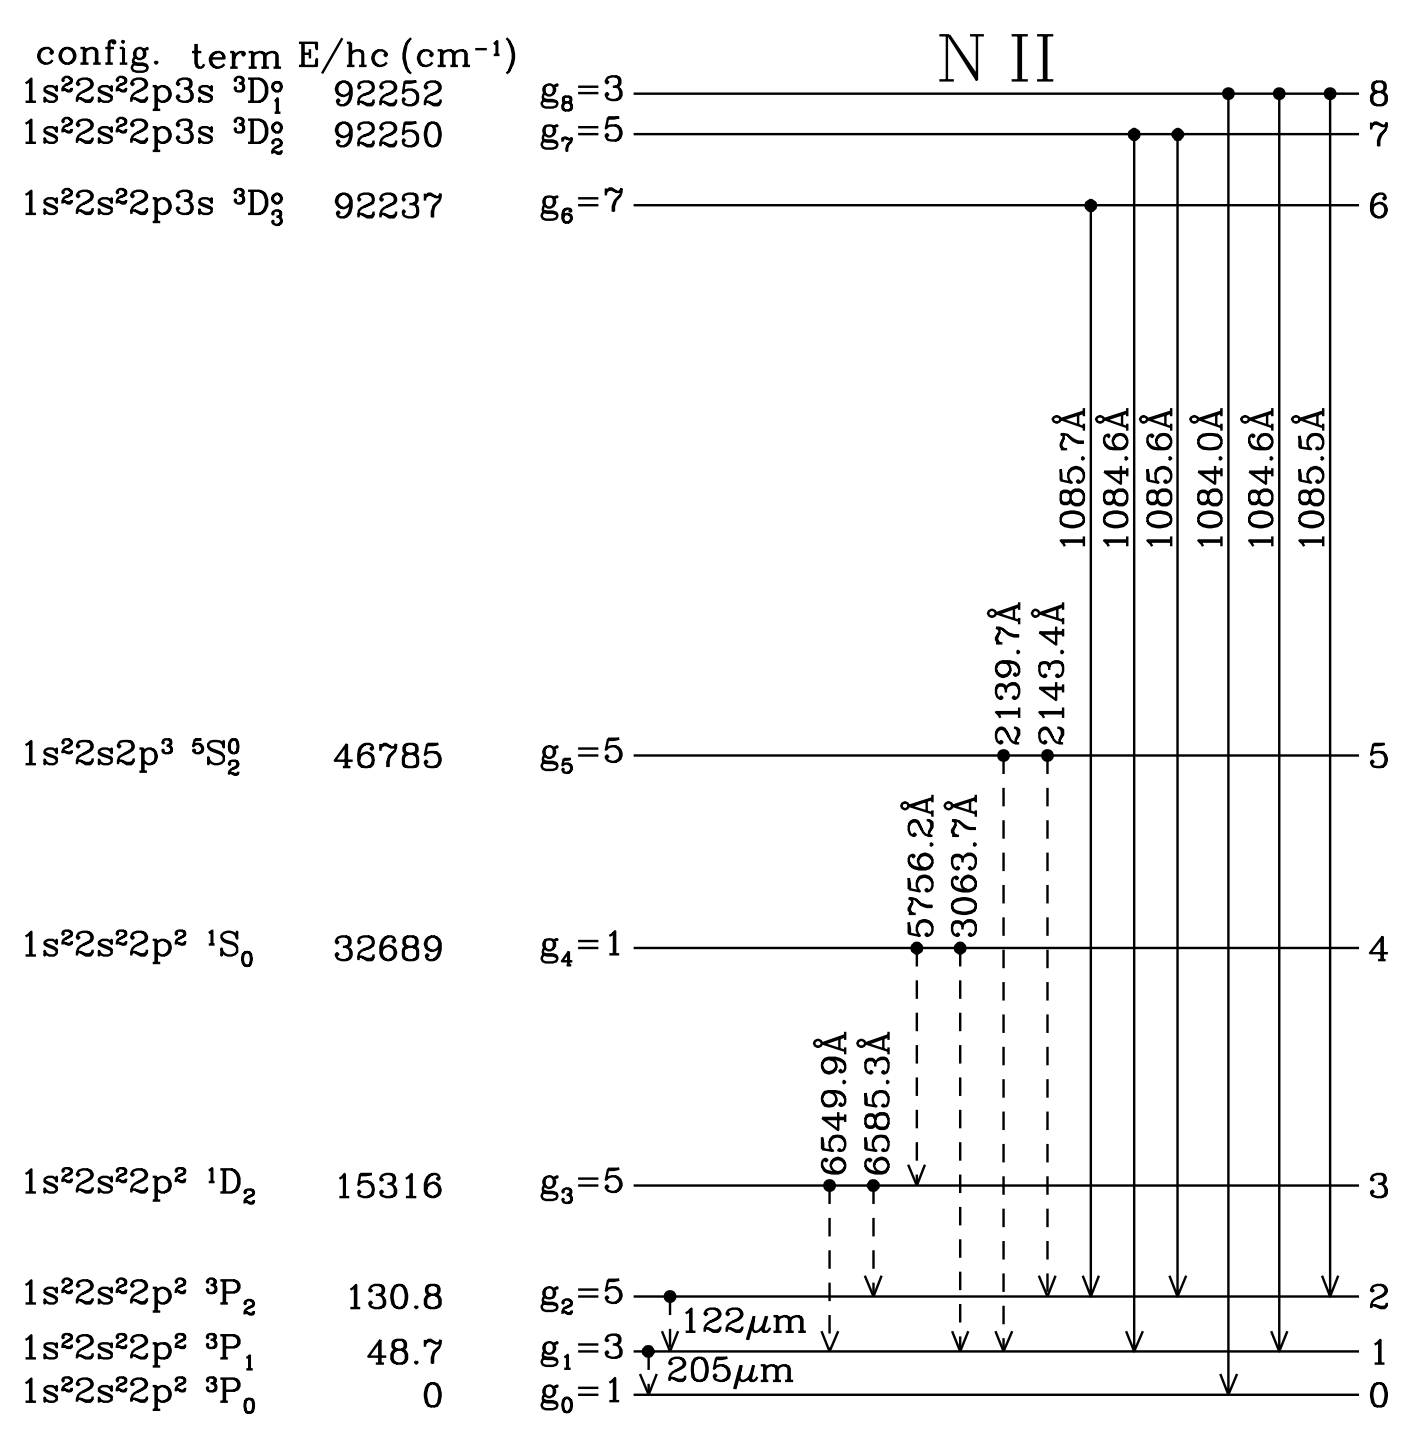
\includegraphics[width=14cm]{figures/NII_levels.png}
    \caption{\footnotesize{First nine energy levels of NII. Forbidden transitions are indicated by broken lines, and allowed transitions by solid lines; forbidden decays are not shown from levels that have permitted decay channels. Fine-structure splitting is not to scale. Hyperfine splitting is not shown. Figure taken from Draine (2015).}}
    \label{fig:NIIlevels}
\end{figure}

{\noindent}\textbf{Allowed: Electric dipole transitions:} The strongest transitions are electric dipole transitions. These are transitions satisfying the following selection rules:

\newpage
\begin{enumerate}
    \item Parity must change.
    \item $\Delta L = 0, \pm1$.
    \item $\Delta J = 0, \pm1$, but $\Delta J = 0\rightarrow0$ is forbidden.
    \item Only one single-electron wave function $n\ell$ changes, with $\Delta\ell=\pm1$.
    \item $\Delta S=0$: Spin does not change.
\end{enumerate}

{\noindent}An allowed transition is denoted \textit{without} square brackets, for example,

\begin{align*}
    {\rm NII}\,1084.0{\rm \AA}\,^3P_0-^3D_1^o.
\end{align*}

{\noindent}This is a transition between the $\ell=1s^22s^22p^2\,3P_0$ and $u=1s^22s^22p3s\,^3D_1^o$ levels of NII, with a wavelength $\lambda_{u\ell}=1084.0$\,\AA. The transition has $A_{u\ell}=2.18\times10^8\,{s^{-1}}$. This decay is very fast -- the lifetime of the $^3D_1^o$ level against this decay is only $1/A_{u\ell}=4.6\,{\rm ns}$!

{\noindent}\textbf{Spin-Forbidden or inter-system transitions:} These are transitions that fulfill the electric dipole selection rules $1$ to $4$ but have $\Delta S\neq0$. These transitions are considerably weaker than allowed transitions. Such transitions are sometimes referred to as \textbf{semi-forbidden}, or \textbf{inter-combination}, or \textbf{inter-system transitions}; the latter is the terminology that we will use. An inter-system transition is denoted with a single right bracket -- for example,

\begin{align*}
    {\rm NII]}\,2143.4{\rm \AA}\,^3P_2-^5S_2^o.
\end{align*}

{\noindent}This is a transition between the $\ell=1s^22s^22p^2\,3P_2$ and $u=1s^22s2p^3\,^5S_2^o$ levels of NII, with a wavelength $\lambda_{u\ell}=2143.4$\,\AA\,and $A_{u\ell}=1.27\times10^2\,{\rm s^{-1}}$.

{\noindent}\textbf{Forbidden transitions:} Forbidden transitions are those that fail to fulfill at least one of the selection rules $1$ to $4$. The transition probabilities vary widely, depending on the values of the electric quadrupole or magnetic dipole matrix elements between the upper and lower states. A forbidden transition is denoted with two square brackets -- for example,

\begin{align*}
    {\rm [NII]}\,6549.9{\rm \AA}\,^3P_1-^1D_2^o.
\end{align*}

{\noindent}This is a transition between the $\ell=1s^22s^22p^2\,3P_1$ and $u=1s^22s^22p^2\,^1D_2^o$ levels of NII, with a wavelength $\lambda_{u\ell}=6549.9$\,\AA\,and $A_{u\ell}=9.20\times10^{-4}\,{\rm s^{-1}}$. This fails rule $1$ (parity is unchanged) and it fails rule $4$ (single electron wave functions are unchanged). This is an example of a \textbf{magnetic dipole transition}.

{\noindent}Another example of a forbidden transition is the \textbf{electric quadrupole transition}

\begin{align*}
    {\rm [NII]}\,5756.2{\rm \AA}\,^1D_2-^1S_0^o.
\end{align*}

{\noindent}This is a transition between the $\ell=1s^22s^22p^2\,1D_2$ and $u=1s^22s^22p^2\,^1S_0^o$ levels of NII, with a wavelength $\lambda_{u\ell}=5756.2$\,\AA\,and $A_{u\ell}=1.17\,{\rm s^{-1}}$. This fails rules $1$ (parity is unchanged) and $4$ (single electron wave functions are unchanged) and it fails rules $2$ and $3$ ($\Delta L=-2$ and $\Delta J=-2$), yet its transition probability is three orders of magnitude larger than the magnetic dipole transition [NII]\,$6549.9$\AA!

{\noindent}We see then that there is a hierarchy in the transition probabilities: very roughly speaking, inter-system lines are $\sim10^6$ times weaker than permitted transitions, and forbidden lines are $\sim10^2-10^6$ times weaker than inter-system transitions.

{\noindent}Despite being very ``weak,'' forbidden transitions are important in astrophysics for the simple reason that every atom and ion has excited states that can only decay via forbidden transitions. At high densities, such excited states would be depopulated by collisions, but at the very low densities of interstellar space, collisions are sufficiently infrequent that there is time for forbidden radiative transitions to take place.

\subsubsection{Follow-up Questions}

\begin{itemize}
    \item Why aren't emission and absorption lines delta functions?
    \item How does this relate to population levels and excitation temperatures?
    \item Are there emission lines in the Sun? Why is there emission from the Calcium doublet?
    \item Write down the heat transfer equation. What do solutions look like?
\end{itemize}

% --------------------------------------------------------------
%               4. 
% --------------------------------------------------------------

\newpage
\subsection{Question 4}

Describe these important sources of stellar opacity: electron scattering, free-free, bound-free, and the H$^-$ ion.

\subsubsection{Short answer}

Answer.

\subsubsection{Additional context}

{\noindent}\textbf{Electron scattering:} If an EM wave passes an electron, the electric field makes the electron oscillate. The oscillating electron represents a classical dipole that radiates in other directions, (i.e., the electron scatters part of the energy of the incoming wave). The weakening of the original radiation due to scattering is equivalent to that by absorption, and we can describe it by way of a cross section at frequency $\nu$ per unit mass ($\kappa_\nu$). This can be calculated classically giving the result

\begin{align*}
    \kappa_\nu = \frac{8\pi}{3} \frac{e_e^2}{\mu_em_u} = 0.20(1+X) ~ [{\rm cm^2\,g^{-1}}],
\end{align*}

{\noindent}where $r_e$ is the classical electron radius, $X$ the mass fraction of hydrogen, and the constant is in ${\rm cm^2\,g^{-1}}$. The term $\mu_em_u$ arises because $\kappa_\nu$ is taken per unit mass; and $\mu_e$ is replaced by (4.30). Since $\kappa_\nu$ does not depend on the frequency, we immediately obtain the \textbf{Rosseland mean for electron scattering}:

\begin{align*}
    \kappa_{\rm sc} = 0.20(1+X) ~ [{\rm cm^2\,g^{-1}}].
\end{align*}

{\noindent}The Thomson scattering just described neglects the exchange of momentum between electron and radiation. If this becomes important, then $\kappa_\nu$ will be reduced compared to the value given above, though this effect plays a role only at temperatures sufficiently high for the scattered photons to be very energetic. In fact, during the scattering process the electron must obtain such a large momentum that its velocity is comparable to $c$, say $v\gtrsim0.1c$ for the equation above to become a bad approximation. The momentum of the photon is $h\nu/c$, which after scattering is partly transferred to the electron, $m_ev\sim h\nu/c$. Therefore relativistic corrections (\textbf{Compton scattering}) become important if the average energy of the photons is $h\nu\gtrsim0.1\,m_ec^2$. For $h\nu$ we take the frequency at which the Planck function has a maximum; then according to Wien's law this is at $h\nu=4.965\,k_BT$, and the full Compton scattering cross section has to be taken into account if $T>0.1\,m_ec^2/(4.965\,{\rm K})$, or roughly $T>10^8\,{\rm K}$. In fact even at $T=10^8\,{\rm K}$ Compton scattering reduces the opacity by only 20\% of that given by the equation above.

{\noindent}\textbf{Free-free:} If during its thermal motion a free electron passes an ion, the two charged particles form a system which can absorb and emit radiation. This mechanism is only effective as long as the electron and ion are sufficiently close. Now, the mean thermal velocity of the electrons is $v\sim\sqrt{T}$, and the time during which they form a system able to absorb or emit is proportional to $1/v\sim1/\sqrt{T}$; therefore, if in a mass element the numbers of electrons and ions are fixed, the number of systems temporarily able to absorb is proportional to $1/\sqrt{T}$.

{\noindent}The absorption properties of such a system have been derived classically; the absorption coefficient per system is proportional to $Z^2\nu^{-3}$, where $Z$ is the charge number of the ion. We therefore expect the absorption coefficient $\kappa_\nu$ of a given mixture of (fully ionized) matter to be

\begin{align*}
    \kappa_\nu \sim Z^2\rho T^{-1/2}\nu^{-3} ~ [{\rm cm^2\,g^{-1}}].
\end{align*}

{\noindent}Here the factor $\rho$ appears because for a given mass element the probability that two particles are accidentally close together is proportional to the density.

{\noindent}For the determination of the Rosseland mean $\kappa$ of this absorption coefficient we make use of a simple theorem: a factor $\nu^\alpha$ contained in $\kappa_\nu$ gives a factor $T^\alpha$ in $\kappa$. With this and the above equation for $\kappa_\nu$ we find

\begin{align*}
    \kappa_{\rm ff} \sim \rho T^{-7/2} ~ [{\rm cm^2\,g^{-1}}].
\end{align*}

{\noindent}All opacities of this form are called \textbf{Kramers opacities} and give only a classical approximation. One normally multiplies the Kramers formula by a correction factor $g$, the so-called \textbf{Gaunt factor}, in order to take care of the quantum-mechanical correction. In the equation for $\kappa_{ff}$, we have still omitted the factor $Z^2$ which appears in $\kappa_\nu$. In general, one has a mixture of different ions, and therefore one has to add the contributions of the different chemical species. The (weighted) sum over the values of $Z^2$ is taken into the constant of proportionality in $\kappa_{ff}$, which then depends on the chemical composition. For a fully ionized mixture a good approximation is given by

\begin{align*}
    \kappa_{ff} = 3.8\times10^{22} (1+X)[(X+Y)+B]\rho T^{-7/2} ~ [{\rm cm^2\,g^{-1}}],
\end{align*}

{\noindent}with the numerical constant in cgs. The mass fractions of H and He are $X$ and $Y$, respectively. Here the factor $(1+X)$ arises, since $\nu_{ff}$ must be proportional to the electron density which is proportional to $(1+X)\rho$. The term $(X+Y)$ in the brackets can be understood in the following way: there are $X/m_u$ hydrogen ions and $Y/(4m_u)$ helium ions. The former have the charge number $1$, the latter the charge number $2$. But since  $\kappa_\nu\sim Z^2$, when adding the contributions of H and He to the total absorption coefficient, we obtain the factor $X/m_u+4Y/(4m_u) = (X_Y)m_u$. Correspondingly the term $B$ gives the contribution of the heavier elements:

\begin{align*}
    B = \sum_i \frac{X_iZ_i^2}{A_i} ~ [{\rm dimensionless}],
\end{align*}

{\noindent}where the summation extends over all elements higher than helium and $A_i$ is the atomic mass number.

{\noindent}\textbf{Bound-free:} We first consider a (neutral) hydrogen atom in its ground state, with an ionization energy of $\chi_0$ (i.e., a photon of energy $h\nu>X_0$ can ionize the atom). Energy conservation then demands that 

\begin{align*}
    h\nu = \chi_0 + \frac{1}{2}m_ev_e^2 ~ [{\rm eV}],
\end{align*}

{\noindent}where $v_e$ is the velocity of the electron released (relative to the ion, which is assumed to be at rest before and after ionization). 

{\noindent}If we define an absorption coefficient $a_\nu$ per ion ($a_\nu=\kappa_\nu\rho/n_{\rm ion}$), we expect $a_\nu=0$ for $\nu<\chi_0/h$ and $a_\nu>0$ for $\nu\geq\chi_0/h$. Classical considerations similar to those which lead to the Kramers dependence of $\kappa_\nu$ for free–free transitions give a $a_\nu\sim\nu^{-3}$ for $\nu\geq\chi_0/h$. Quantum-mechanical corrections can again be taken into account by a Gaunt factor. But if we have neutral hydrogen atoms in different stages of excitation, the situation is different: an atom in the first excited stage has an absorption coefficient $a_\nu=0$ for $h\nu<\chi_1$, where $\chi_1$ is the energy necessary to ionize a hydrogen atom from the first excited state, while $a_\nu\sim\nu^{-3}$ for $h\nu\geq\chi_1$. The absorption coefficient $\kappa_\nu$ for a mixture of hydrogen atoms in different states of excitation is a superposition of the $a_\nu$ for different stages of excitation. The resulting $\kappa_\nu$ is a saw-tooth function. In order to obtain $\kappa_\nu$ for a certain value of the temperature $T$, one has to determine the relative numbers of atoms in the different stages of excitation by the Boltzmann formula; then their absorption coefficients $a_\nu$, weighted with their relative abundances, are to be summed.

{\noindent}If there are ions of different chemical species with different degrees of ionization, one has to sum the functions $a_\nu$ for all species in all stages of excitation and all degrees of ionization before carrying out the Rosseland integration. An important source of opacity are bound-free transitions of neutral hydrogen atoms, in which case the opacity must be proportional to the number of neutral hydrogen atoms and $\kappa$ can be written in the form

\begin{align*}
    \kappa_{bf} = X(1-x)\tilde{\kappa}(T) ~ [{\rm cm^2\,g^{-1}}].
\end{align*}

{\noindent}Here $\tilde{\kappa}(T)$ is obtained by Rosseland integration over (weighted) sums of functions $a_\nu$ for the different stages of excitation, while $x$ is the degree of ionization.

{\noindent}\textbf{H$^-$ ion:} Hydrogen atom has a bound state for a second electron in the field of the proton, though it has a very low ionization potential, $E_{{\rm H}^-}=0.75\,{\rm eV}$. The number density of negative hydrogen ions will be proportional to the electron density, which, in all but the most metal-poor stars, will be set by ionization of the metals (which have much lower ionization potentials that hydrogen and helium). Thus, the H$^-$ opacity will scale as $\kappa_{{\rm H}^-} \propto \rho XZ$ at low temperatures; H$^-$ is of course easily ionized at higher temperatures, and at very low temperatures even metals will not be ionized, so there will be no electrons to form H$^-$ by combining with H.

% --------------------------------------------------------------
%               5. 
% --------------------------------------------------------------

\newpage
\subsection{Question 5}

Describe the processes that can cause pulsations in a star’s luminosity, and provide at least one example of a class of stellar pulsation.

\subsubsection{Short answer}

Answer.

\subsubsection{Additional context}

Additional context.

\subsubsection{Follow-up Questions}

\begin{itemize}
    \item What about the instability strip? RR Lyrae?
    \item What is the period-luminosity relation?
    \item What is the form of the period-luminosity relation?
    \item How would you derive the time scale of pressure waves in a star?
    \item How would you order-of-magnitude estimate the period for a pulsation?
\end{itemize}

% --------------------------------------------------------------
%               6. 
% --------------------------------------------------------------

\newpage
\subsection{Question 6}

Briefly describe the sources of thermal energy for stars and planets.

\subsubsection{Short answer}

The sources of thermal energy of stars include:

\begin{itemize}
    \item \textbf{gravitational energy}:
    \item \textbf{rotational energy}: 
    \item \textbf{nuclear energy}:
\end{itemize}

{\noindent}The sources of thermal energy of planets include:

\begin{itemize}
    \item \textbf{radioactive decay}:
    \item \textbf{differentiation}: 
    \item \textbf{solar radiation}:
    \item \textbf{accretion/impact}:
    \item \textbf{tidal heating}:
\end{itemize}

\subsubsection{Additional context}

{\noindent}\textbf{Stars:}

{\noindent}One of the great mysteries of the late nineteenth and early twentieth centuries was the source of the energy required to sustain the luminosity of the sun. By then, the defining Solar parameters of mass, radius, and luminosity were known with sufficient precision to attempt to relate them. For instance, it was clear that if the Sun derived its energy from chemical processes typically yielding less that $10^{12}\,{\rm erg\,g^{-1}}$, it could shine no longer than about $10,000$ years at its current luminosity. It is said that Lord Kelvin, in noting that the liberation of gravitational energy could only keep the sun shining for about $10$ million years, found it necessary to reject Charles Darwin's theory of evolution because there would have been insufficient time for natural selection to provide the observed diversity of species.

{\noindent}\textbf{Gravitational energy:} It is generally conceded that the Sun has shone at roughly its present luminosity for at least the past $2$ billion years and has been in existence for nearly $5$ billion years. With this in mind, let us begin our study of the sources of stellar energy with an inventory of the stores of energy available to the sun. Perhaps the most obvious source of energy is that suggested by Lord Kelvin, namely gravitation:

\begin{align*}
    E_p \leq -\frac{3}{5}\frac{GM^2}{R} ~ [{\rm J}].
\end{align*}

{\noindent}The right-hand side of the inequality is the gravitational potential energy for a uniform density sphere, which provides a sensible upper limit for the energy. Remember that the gravitational energy is considered negative by convention; a rather larger magnitude of energy may be available for a star that is more centrally concentrated than a uniform-density sphere. We may acquire a better estimate of the gravitational potential energy by using the results for a polytrope. Chandrasekhar obtains the following result for the gravitational potential energy of a polytrope:

\begin{align*}
    E_p = -\frac{3}{5-n}\frac{GM^2}{R} ~ [{\rm J}].
\end{align*}

{\noindent}For a star in convective equilibrium (that is, $n=3/2$) the factor multiplying $GM^2/R$ becomes $6/7$ or nearly unity. Note that for a polytrope of index $5$, $U_g\rightarrow-\infty$ implying an infinite central concentration of material. This is also one of the polytropes for which there exists an analytic solution. Thus, one has the picture of a mass point surrounded by a massless envelope of infinite extent. This equation also tells us that as the polytropic index increases, so does the central concentration.

{\noindent}It is not at all obvious that the total gravitational energy would be available to permit the star to shine. Some energy must be provided in the form of heat, to provide the pressure which supports the star. We may use the Virial theorem [equation (1.2.35)] to estimate how much of the gravitational energy can be utilized by the luminosity. Consider a star with no mass motions, so that the macroscopic kinetic energy T in equation (1.2.35) is zero. Let us also assume that the equilibrium state is good enough that we can replace the time averages by the instantaneous values. Then the \textbf{Virial theorem becomes}

\begin{align*}
    2E_k+E_p = 0 ~ [{\rm J}].
\end{align*}

{\noindent}Recall that $E_k$ is the total internal kinetic energy of the gas which includes all motions of the particles making up the gas. Now we know from thermodynamics that not all the internal kinetic energy is available to do work, and it is therefore not counted in the internal energy of the gas.

{\noindent}For simplicity, let us assume that $\gamma$ is constant through out the star. Remembering that the total energy $E$ is the sum of the internal energy and the gravitational energy, we can express the Virial theorem in the following ways:

\begin{align*}
    E_k &= -\frac{E_p}{3(\gamma-1)} ~ [{\rm J}]\\
    E_{\rm tot} &= -(3\gamma-4)E_{\rm th} ~ [{\rm J}]\\
    E_{\rm tot} &= \frac{3\gamma-4}{3(\gamma-1)}E_p ~ [{\rm J}].
\end{align*}

{\noindent}It is clear that for $\gamma>4/3$ (that is, $n<3$), the total energy of the star will be negative. This simply says that the star is gravitationally bound and can be in equilibrium. So we can look for the physically reasonable polytropes to have indices less than or equal to $3$. The case of $n=3$ is an interesting one for it represents radiation dominated gas. In the limit of complete radiation dominance, the total energy of the configuration will be zero.

{\noindent}\textbf{Rotational energy:} Stars do rotate, and we should not forget to count the rotational energy in the inventory of energies. We may place a reasonable upper limit on the magnitude of the rotational energy that we can expect by noting that (1) the moment of inertia of the star will always be less than that of a sphere of uniform density and (2) there is a limit to the angular velocity $\omega_c$ at which the star can rotate. Thus, for a centrally condensed star

\begin{align*}
    \omega^2 &= \frac{8GM}{27R^3} ~ [{\rm km^2\,s^{-2}\,kpc^{-2}}] \\
    I_z &< \frac{2}{5}MR^2 ~ [{\rm kg\,km^2}],
\end{align*}

{\noindent}which implies that the rotational energy must be bounded by

\begin{align*}
    E_{\rm rot} = \frac{1}{2}I_z\omega^2 < \frac{8}{135}\frac{GM^2}{R} ~ [{\rm J}].
\end{align*}

{\noindent}One may quibble that we have used the angular velocity limit for a centrally condensed star and the moment of inertia for a uniform-density star, but the fact remains that it is extremely difficult for a star to have more than about 10 percent of the magnitude of its gravitational energy stored in the form of rotational energy.

{\noindent}\textbf{Nuclear energy:} Of course, the ultimate upper limit for stored energy is the energy associated with the rest mass itself. It is also the common way of estimating the energy available from nuclear sources. Indeed, that fraction of the rest mass which becomes energy when four hydrogen atoms are converted to one helium atom provides the energy to sustain the solar luminosity. Below in Table \ref{table:solarenergy} is a short table giving the mass loss for a few common elements involved in nuclear fusion processes.

\begin{table}[h]
    \centering
    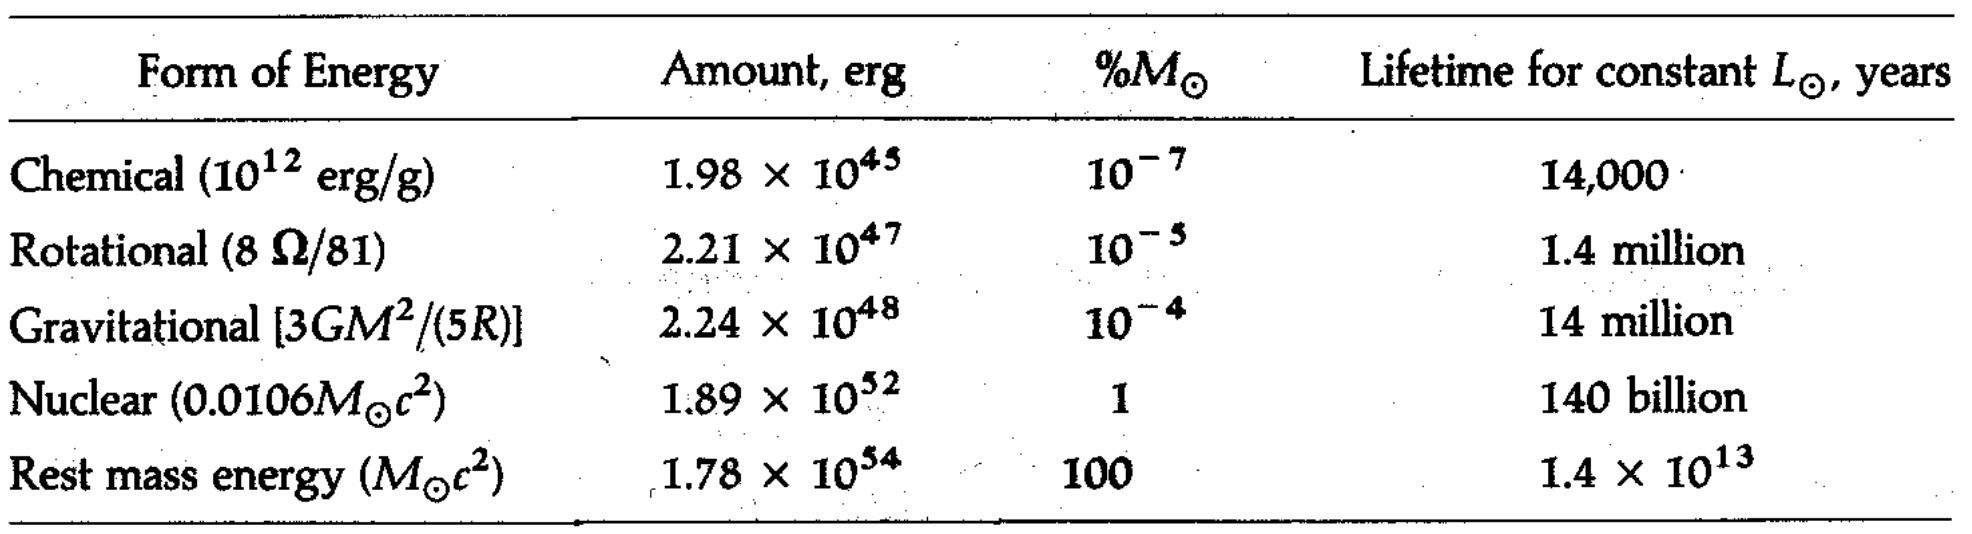
\includegraphics[width=14cm]{figures/SolarEnergy.png}
    \caption{\footnotesize{Possible sources of Solar energy. Table taken from Kippenhahn, Weigert \& Weiss (2012).}}
    \label{table:solarenergy}
\end{table}

{\noindent}Clearly most of the energy to be gained from nuclear fusion occurs by the conversion of hydrogen to helium and less than one-half of that energy can be obtained by all other fusion processes that carry helium to iron. Nevertheless, $0.7\%$ of $mc^2$ is a formidable supply of energy. Table \ref{table:solarenergy} is a summary of the energy that one could consider as being available to the Sun. All these entries are generous upper limits. For example, the sun rotates at less than $0.5\%$ of its critical velocity, it was never composed of $100\%$ hydrogen and will begin to change significantly when a fraction of the core hydrogen is consumed, and not all the gravitational energy could ever be converted to energy for release. In any event, only nuclear processes hold the promise of providing the solar luminosity for the time required to bring about agreement with the age of the solar system as derived from rocks and meteorites. However, the time scales of Table \ref{table:solarenergy} are interesting because they provide an estimate of how long the various energy sources could be expected to maintain some sort of equilibrium configuration.

{\noindent}\textbf{Planets:}

\subsubsection{Follow-up Questions}

\begin{itemize}
    \item Why do different nuclear reaction pathways have different temperature sensitivities?
    \item If I assume a constant core temperature on the main sequence, how does stellar radius depend on mass?
    \item What are some other thermal sources, like say for neutron stars?
\end{itemize}

% --------------------------------------------------------------
%               7. 
% --------------------------------------------------------------

\newpage
\subsection{Question 7}

Describe the process by which supernovae produce light. Why are Type Ia supernovae generally brighter than Type II events?

\subsubsection{Short answer}

Answer.

\subsubsection{Additional context}

Additional context.

\subsubsection{Follow-up Questions}

\begin{itemize}
    \item When a star goes supernova, how much of the luminous energy generated at the rebound is available for heating the gas? As in, where does the heat come from?
    \item Are there cases where the rebound shock wave can't blow up the star? Why, and what happens then?
\end{itemize}

% --------------------------------------------------------------
%               8. 
% --------------------------------------------------------------

\newpage
\subsection{Question 8}

Describe the condition for a star’s envelope to become convective. Why are low mass stars convective in their outer envelopes while high mass stars are convective in their inner cores?

\subsubsection{Short answer}

The radiation pressure gradient is given by 

\begin{align*}
    \frac{{\rm d}P_{\rm rad}}{{\rm d}r} = -\frac{\kappa\rho}{c}F_{\rm rad} ~ [{\rm P\,m}],
\end{align*}

{\noindent}where $F_{\rm rad}$ is the outward radiative flux. The radiation pressure may also be expressed as

\begin{align*}
    \frac{{\rm d}P_{\rm rad}}{{\rm d}r} = \frac{4}{3} aT^3 \frac{{\rm d}T}{{\rm d}r} ~ [{\rm P\,m}].
\end{align*}

{\noindent}Equating the two, we have

\begin{align*}
    \frac{{\rm d}T}{{\rm d}r} = -\frac{3}{4ac}\frac{\kappa\rho}{T^3}F_{\rm rad} ~ [{\rm K\,m^{-1}}].
\end{align*}

{\noindent}If we use the expression for the radiative flux written in terms of the local radiative luminosity of the star at radius $r$, 

\begin{align*}
    F_{\rm rad} = \frac{L_r}{4\pi r^2} ~ [{\rm erg\,s^{-1}\,cm^{-2}}],
\end{align*}

{\noindent}the temperature gradient for radiative transport becomes

\begin{align*}
    \frac{{\rm d}T}{{\rm d}r} = -\frac{3}{4ac}\frac{\kappa\rho}{T^3}\frac{L_r}{4\pi r^2} ~ [{\rm K\,m^{-1}}].
\end{align*}

{\noindent}As either the flux or the opacity increases, the temperature gradient must become steeper (i.e., more negative) if radiation transport is to carry all of the required luminosity outward. The same situation holds as the density increases or the temperature increases.

{\noindent}We now consider a situation where a hot convective bubble of gas rises and expands \textbf{adiabatically}, meaning that the bubble does not exchange heat with its surroundings. After it has travelled some distance, it finally \textbf{thermalizes}, giving up any excess heat as it loses its identity and dissolves into the surrounding gas. Differentiating the \textbf{ideal gas law}

\begin{align*}
    P = \frac{\rho k_BT}{\mu m_{\rm H}} ~ [{\rm P}]
\end{align*}

{\noindent}yields an expression involving the bubble's \textbf{temperature gradient}

\begin{align*}
    \frac{{\rm d}P}{{\rm d}r} = -\frac{P}{\mu}\frac{{\rm d}\mu}{{\rm d}r} + \frac{P}{\rho}\frac{{\rm d}\rho}{{\rm d}r} + \frac{P}{T}\frac{{\rm d}T}{{\rm d}r}.
\end{align*}

{\noindent}Using the adiabatic relationship between pressure and density

\begin{align*}
    PV^\gamma = K ~ [{\rm P\,m^3}]
\end{align*}

{\noindent}and recalling that $V\equiv1/\rho$ is the \textbf{specific volume}, we have that

\begin{align*}
    P = K\rho^\gamma ~ [{\rm P}].
\end{align*}

{\noindent}Differentiating and re-writing, we obtain

\begin{align*}
    \frac{{\rm d}P}{{\rm d}r} = \gamma \frac{P}{\rho}\frac{{\rm d}\rho}{{\rm d}r} ~ [{\rm P\,m^{-1}}].
\end{align*}

{\noindent}If we assume for simplicity that the mean molecular weight $\mu$ is constant, we can combing equations for ${\rm d}P/{\rm d}r$ to give the \textbf{adiabatic temperature gradient}

\begin{align*}
    \left(\frac{{\rm d}T}{{\rm d}r}\right)_{\rm ad} = \left(1-\frac{1}{\gamma}\right) \frac{T}{P}\frac{{\rm d}P}{{\rm d}r} ~ [{\rm K\,m^{-1}}].
\end{align*}

{\noindent}Using the equation of \textbf{hydrostatic equilibrium}

\begin{align*}
    \frac{{\rm d}P}{{\rm d}r} = -\frac{GM_r\rho}{r^2} = -\rho g ~ [{\rm P\,m^{-1}}], ~~~ g \equiv \frac{GM_r}{r^2} ~ [{\rm m\,s^{-2}}]
\end{align*}

{\noindent}and the ideal gas law, we finally obtain

\begin{align*}
    \left(\frac{{\rm d}T}{{\rm d}r}\right)_{\rm ad} = \left(1-\frac{1}{\gamma}\right) \frac{\mu m_{\rm H}}{k}\frac{GM_r}{r^2} ~ [{\rm K\,m^{-1}}].
\end{align*}

{\noindent}If the star's actual temperature gradient is \textit{steeper} than the adiabatic temperature gradient,

\begin{align*}
    \left\lvert\frac{{\rm d}T}{{\rm d}r}\right\rvert_{\rm act} > \left\lvert\frac{{\rm d}T}{{\rm d}r}\right\rvert_{\rm ad} ~ [{\rm K\,m^{-1}}],
\end{align*}

{\noindent}the temperature gradient is said to be \textbf{super-adiabatic} (recall that ${\rm d}T/{\rm d}r<0$). In the deep interior of a star, if the actual temperature gradient is just \textit{slightly} larger than the adiabatic temperature gradient, this may be sufficient to carry nearly all of the luminosity by convection. Consequently, it is often the case that either radiation or convection dominates the energy transport in the deep interior of stars, while the other energy transport mechanism contributes very little to the total energy outflow. The particular mechanism in operation is determined by the temperature gradient. However, near the surface of the star, the situation is much more complicated: both radiation and convection can carry significant amounts of energy simultaneously.

{\noindent}In general, convection will occur when

\begin{enumerate}
    \item the stellar opacity is large, implying that an unchievably steep temperature gradient would be necessary for radiative transport;
    \item a region exists where ionization is occurring, causing a large specific heat and a low adiabatic temperature gradient; and
    \item the temperature dependence of the nuclear energy generation rate is large, causing a steep radiative flux gradient and a large temperature gradient.
\end{enumerate}

{\noindent}In the atmosphere of many stars, the first two conditions can occur simultaneously, whereas the third condition would occur only deep in stellar interiors. In particular, the third condition can occur when the highly temperature-dependent CNO cycle or triple alpha processes are occuring.

\subsubsection{Additional context}

Three different energy transport mechanisms operate in stellar interiors. \textbf{Radiation} allows the energy produced by nuclear reactions and gravitation to be carried to the surface via photons, the photons being absorbed and re-emitted in nearly random directions as they encounter matter. This suggests that the opacity of the material must play an important role, as one would expect. \textbf{Convection} can be a very efficient transport mechanism in many regions of a star, with hot, buoyant mass elements carrying excess energy outward while cool elements fall inward. Finally, \textbf{conduction} transports heat via collisions between particles. Although conduction can play an important role in some stellar environments, it is generally insignificant in most stars throughout the majority of their lifetimes. 

{\noindent}\textbf{Radiative transport of energy: basic estimates} Rough estimates show important features of the radiative transfer in stellar interiors and justify an enormous simplification of the formalism. Let us first estimate the mean free path $\ell_{\rm mfp}$ of a photon at an ``average'' point inside a star like the Sun:

\begin{align*}
    \ell_{\rm mfp} = \frac{1}{\kappa\rho} ~ [{\rm m}].
\end{align*}

{\noindent}where $\kappa$ is a mean absorption coefficient (i.e., a radiative cross section per unit mass averaged over frequency). Typical values for stellar material are of order $\kappa\approx1\,{\rm cm^2\,g^{-1}}$; for the ionized hydrogen in stellar interiors, a lower limit is certainly the value for electron scattering, $\kappa\approx0.4\,{\rm cm^2\,g^{-1}}$. Using this and the mean density of matter in the Sun, $\bar{\rho}_\odot=1.4\,{\rm g\,cm^{-3}}$, we obtain a mean free path of only

\begin{align*}
    \ell_{\rm mfp} = \frac{1}{\kappa\rho} = \frac{1}{1\,{\rm cm^2\,g^{-1}}\cdot0.4\,{\rm g\,cm^{-3}}} \approx2 ~ [{\rm cm}],
\end{align*}

{\noindent}i.e., stellar matter is very opaque.

{\noindent}The typical temperature gradient in the star can be roughly estimated by averaging between centre ($T_c\approx10^7\,{\rm K}$) and surface ($T_0\approx10^4\,{\rm K}$):

\begin{align*}
    \frac{\Delta T}{\Delta r} \approx \frac{T_c-T_0}{R_\odot} \approx 1.4\times10^{-4}\,[{\rm K\,cm^{-1}}].
\end{align*}

{\noindent}The radiation field at a given point is emitted from a small, nearly isothermal surrounding, the differences of temperature being only of order $\Delta T=\ell_{\rm mfp}({\rm d}T/{\rm d}r)\approx3\times10^{-4}\,{\rm K}$. Since the energy density of radiation is $u\sim T^4$, the relative anisotropy of the radiation at a point with $T=10^7\,{\rm K}$ is $\Delta T/T\sim10^{-10}$. The situation in stellar interiors must obviously be very close to TE, and the radiation very close to that of a blackbody. Nevertheless, the small remaining anisotropy can easily be the carrier of the stars' huge luminosity: this fraction of $10^{-10}$ of the flux emitted from ${\rm 1\,cm^2}$ of a blackbody of $T=10^7\,{\rm K}$ is still $10^3$ times larger than the flux at the solar surface ($6\times10^{10}\,{\rm erg\,cm^{-2}\,s^{-1}}$. Radiative transport of energy occurs via the non-vanishing net flux (i.e., via the surplus of the outwards-going radiation emitted from somewhat hotter material below over the inwards-going radiation emitted from less-hot material above).

{\noindent}\textbf{Diffusion of radiative energy:} The above estimates have shown that for radiative transport in stars, the mean free path $\ell_{\rm mfp}$ of the ``transporting particles'' (i.e., photons) is very small compared to the characteristic length $R$ (stellar radius) over which the transport extends: $\ell_{\rm mfp,\odot}/R_\odot\approx3\times10^{-11}$. In this case, the transport can be treated as a diffusion process, which yields an enormous simplification of the formalism. We derive the corresponding equation by analogy to those for particle diffusion.

{\noindent}The diffusive flux $j$ of particles (per unit area and time) between places of different particle density $n$ is given by

\begin{align*}
    \vec{j} = -D\nabla n ~ [{\rm ???}],
\end{align*}

{\noindent}where $D$ is the coefficient of diffusion,

\begin{align*}
    D = \frac{1}{3}v\ell_{\rm mfp} ~ [{\rm s^{-1}}],
\end{align*}

{\noindent}determined by the average values of mean velocity $v$ and mean free path $\ell_{\rm mfp}$ of the particles.

{\noindent}In order to obtain the corresponding diffusive flux of radiative energy $\vec{F}$; we replace $n$ by the energy density of radiation $U$;

\begin{align*}
    u = aT^4 = \frac{4\sigma}{c}T^4 ~ [{\rm erg\,cm^{-3}}].
\end{align*}

{\noindent}Here, $a=7.57\times10^{-15}\,{\rm erg\,cm^{3}\,K^{-4}}$ is the \textbf{radiation density constant}. Owing to the spherical symmetry of the problem, $\vec{F}$ has only a radial component $F_r=\lvert\vec{F}\rvert=F$ and $\nabla U$ reduces to the derivative in the radial direction

\begin{align*}
    \frac{\partial u}{\partial r} = 4aT^3\frac{\partial T}{\partial r} ~ [{\rm erg\,cm^{-4}}].
\end{align*}

{\noindent}Using this result along with the equation for $\vec{j}$, this immediately gives us

\begin{align*}
    F = - \frac{4ac}{3} \frac{T^3}{\kappa\rho} \frac{\partial T}{\partial r} ~ [{\rm erg\,s^{-1}\,cm^{-2}}].
\end{align*}

{\noindent}Note that this can be interpreted formally as an \textbf{equation for heat conduction} by writing

\begin{align*}
    \vec{F} = -k_{\rm rad}\nabla T ~ [{\rm erg\,s^{-1}\,cm^{-2}}],
\end{align*}

{\noindent}where 

\begin{align*}
    k_{\rm rad} = \frac{4ac}{3} \frac{T^3}{\kappa\rho} ~ [{\rm erg\,cm^{-1}\,K^{-1}\,s^{-1}}]
\end{align*}

{\noindent}represents the \textbf{coefficient of conduction} for this radiative transport.

{\noindent}We solve $F$ for the gradient of the temperature and replace it by the usual local luminosity $L=4\pi r^2F$; then

\begin{align*}
    \frac{\partial T}{\partial r} = - \frac{3}{16\pi ac} \frac{\kappa\rho L}{r^2T^3} ~ [{\rm K\,cm^{-1}}]
\end{align*}

{\noindent}Of course, this neat and simple equation becomes invalid when one approaches the surface of the star. Because of the decreasing density, the mean free path of the photons will there become comparable with (and finally larger than) the remaining distance to the surface; hence the whole diffusion approximation breaks down, and one has to solve the far more complicated full set of transport equations for radiation in the stellar atmosphere (these equations indeed yield our simple diffusion approximation as the proper limiting case for large optical depths).

{\noindent}\textbf{The Rosseland mean for $\kappa_\nu$:} The above equations are independent of the frequency $\nu$; $F$ and $L$ are quantities integrated over all frequencies, so that the quantity   must represent a ``proper mean'' over $\nu$. We shall now prescribe a method for this averaging.

{\noindent}In general the absorption coefficient depends on the frequency $\nu$. Let us denote this by adding a subscript $\nu$ to all quantities that thus become frequency dependent: $\kappa_\nu$, $\ell_\nu$, $D_\nu$, $u_\nu$ etc.

{\noindent}For the diffusive energy flux $\vec{F}_\nu$ of radiation in the interval $[\nu,\nu+{\rm d}\nu]$, we write now

\begin{align*}
    \vec{F}_\nu &= -D_\nu \nabla u_\nu ~ [{\rm erg\,s^{-1}\,cm^{-2}}], \\
    D_\nu &= \frac{1}{3}c\ell_\nu = \frac{c}{3\kappa_\nu\rho} ~ [{\rm m^2\,s^{-1}}],
\end{align*}

{\noindent}while the energy density in the same interval is given by

\begin{align*}
    u_\nu = \frac{4\pi}{c}B(\nu,T) = \frac{8\pi h}{c^3} \frac{\nu^3}{e^{h\nu/k_BT}-1}  ~ [{\rm erg\,cm^{-3}}].
\end{align*}

{\noindent}$B(\nu,T)$ denotes here the \textbf{Planck function} for the intensity of blackbody radiation (differing from the usual formula for the energy density simply by the factor $4\pi/c$. From this equation for $u_\nu$, we have

\begin{align*}
    \nabla u_\nu = \frac{4\pi}{c} \frac{\partial B}{\partial T}\nabla T,
\end{align*}

{\noindent}which together with $D_\nu$ is inserted into  $F_\nu$, the latter then being integrated over all frequencies to obtain the total flux $F$: 

\begin{align*}
    \vec{F} = -\left[ \frac{4\pi}{3\rho} \int\limits_0^\infty \frac{1}{\kappa_\nu} \frac{\partial B}{\partial T} {\rm d}\nu \right] \nabla T ~ [{\rm m^2\,s^{-1}}].
\end{align*}

{\noindent}We have thus regained $\vec{F}=-k_{\rm rad}\nabla T$ with

\begin{align*}
    k_{\rm rad} = \frac{4\pi}{3\rho} \int\limits_0^\infty \frac{1}{\kappa_\nu} \frac{\partial B}{\partial T} {\rm d}\nu ~ [{\rm erg\,cm^{-1}\,K^{-1}\,s^{-1}}].
\end{align*}

{\noindent}Equating this expression for $k_{\rm rad}$ with that in the averaged form, we have immediately the proper formula for averaging the absorption coefficient:

\begin{align*}
    \frac{1}{\kappa} = \frac{\pi}{acT^3} \int\limits_0^\infty \frac{\partial B}{\partial T} {\rm d}\nu ~ [{\rm cm^2\,g^{-1}}].
\end{align*}

{\noindent}This s the so-called \textbf{Rosseland mean}. Since

\begin{align*}
    \int\limits_0^\infty \frac{\partial B}{\partial T}{\rm d}\nu = \frac{acT^3}{\pi},
\end{align*}

{\noindent}the Rosseland mean is formally the harmonic mean of    with the weighting function $\partial B/\partial T$, and it can simply be calculated, once the function $\kappa_\nu$ is known from atomic physics.

{\noindent}In order to see the physical interpretation of the Rosseland mean, we rewrite $\vec{F}_\nu=-D_\nu\nabla u_\nu$ as

\begin{align*}
    \vec{F}_\nu = -\left(\frac{1}{\kappa_\nu}\frac{\partial B(\nu,T)}{\partial T}\right)\frac{4\pi}{3\rho}\nabla T ~ [{\rm m^2\,s^{-1}}].
\end{align*}

{\noindent}This shows that, for a given point in the star ($\rho$ and $\nabla T$ given), the integrand in $1/\kappa$ is at all frequencies proportional to the net flux $\vec{F}_\nu$ of energy. The Rosseland mean therefore favours the frequency ranges of maximum energy flux. One could say that an average \textit{transparency} is evaluated rather than an \textit{opacity} -- which is plausible, since it is to be used in an equation describing the transfer of energy rather than its blocking.

{\noindent}One can also easily evaluate the frequency where the weighting function $\partial B/\partial T$ has its maximum. One finds that, for given a temperature, $\partial B/\partial T\sim x^4e^x(e^x-1)^{-2}$ with $x=h\nu/k_BT$. Differentiation with respect to $x$ shows that the maximum of $\partial B/\partial T$ is close to $x=4$.

{\noindent}The way we have defined the Rosseland mean $\kappa$, which is a kind of weighted harmonic mean value, has the uncomfortable consequence that the opacity $\kappa$ of a mixture of two gases having the opacities $\kappa_1,\kappa_2$ is not the sum of the opacities: $\kappa\neq\kappa_1\kappa_2$. Therefore, in order to find $\kappa$ for a mixture containing the weight fractions $X$ of hydrogen and $Y$ of helium, the mean opacities of the two single gases are of no use. Rather one has to add the frequency-dependent opacities $\kappa_\nu=X_{\kappa_\nu,{\rm H}}+Y_{\kappa_\nu,{\rm He}}$ before calculating the Rosseland mean. For any new abundance ratio $X/Y$ the averaging over the frequency has to be carried out separately.

{\noindent}In the above we have characterized the energy flux due to the diffusion of photons by $F_\nu$. Since in the following we shall encounter other mechanisms for energy transport, from now on we shall specify this radiative flux by the vector $\vec{F}_{\rm rad}$. Correspondingly we shall use $\kappa_{\rm rad}$ instead of  $\kappa$, etc.

{\noindent}\textbf{Conductive transport of energy:} In heat conduction, energy transfer occurs via collisions during the random thermal motion of the particles (electrons and nuclei in completely ionized matter, otherwise atoms or molecules). A basic estimate shows that in ``ordinary'' stellar matter (i.e., in a non-degenerate gas), conduction has no chance of taking over an appreciable part of the total energy transport. Although the collisional cross sections of these charged particles are rather small at the high temperatures in stellar interiors $(10^{-18}-10^{-20}\,cm^2$ per particle), the large density ($\rho=1.4\,{\rm g\,cm^{-3}}$ in the Sun) results in mean free paths several orders of magnitude less than those for photons; and the velocity of the particles is only a few per cent of $c$. Therefore the coefficient of diffusion is much smaller than that for photons.

{\noindent}The situation becomes quite different, however, for the cores of evolved stars where the electron gas is highly degenerate. The density can be as large as $10^6\,{\rm g\,cm^{-3}}$. But degeneracy makes the electrons much faster, since they are pushed up close to the Fermi energy; and degeneracy increases the mean free path considerably, since the quantum cells of phase space are filled up such that collisions in which the momentum is changed become rather improbable. Then the coefficient of diffusion (which is proportional to the product of mean free path and particle velocity) is large, and heat conduction can become so efficient that it short-circuits the radiative transfer.

{\noindent}The energy flux $\vec{F}_{\rm cd}$ due to heat conduction may be written as

\begin{align*}
    \vec{F}_{\rm cd} = -k_{\rm cd}\nabla T ~ [{\rm m^2\,s^{-1}}].
\end{align*}

{\noindent}The sum of the conductive flux $\vec{F}_{\rm cd}$ and the radiative flux $\vec{F}_{\rm rad}$ is

\begin{align*}
    \vec{F} = \vec{F}_{\rm rad}+\vec{F}_{\rm cd} = -(k_{\rm rad}+k_{\rm cd})\nabla T ~ [{\rm m^2\,s^{-1}}],
\end{align*}

{\noindent}On the other hand, we can just as well write the conductive coefficient $k_{\rm cd}$ formally in analogy to $k_{\rm rad}$ as

\begin{align*}
    k_{\rm cd} = \frac{4ac}{3}\frac{T^3}{\kappa_{\rm cd}\rho} ~ [{\rm cm^2\,g^{-1}}],
\end{align*}

{\noindent}hence defining the \textbf{conductive opacity} $\kappa_{\rm cd}$. Then the flux becomes

\begin{align*}
    \vec{F} = -\frac{4ac}{3}\frac{T^3}{\rho} \left(\frac{1}{\kappa_{\rm rad}}+\frac{1}{\kappa_{\rm cd}}\right) \nabla T,
\end{align*}

{\noindent}which shows that we arrive formally at the same type of equation as in the pure radiative case if we replace $1/\kappa$ by $1/\kappa_{\rm rad}+1/\kappa_{\rm cd}$. Again the result is plausible, since the mechanism of transport that provides the largest flux will dominate the sum (i.e., the mechanism for which the stellar matter has the highest ``transparency'').

{\noindent}The basic equation for energy transport which, if we define properly, holds for radiative and conductive energy transport, can be rewritten in a convenient form. Starting with

\begin{align*}
    \frac{\partial T}{\partial r} = - \frac{3}{16\pi ac} \frac{\kappa\rho L}{r^2T^3} ~ [{\rm K\,cm^{-1}}],
\end{align*}

{\noindent}we can transform to the independent variable mass $m$ using the fact that $\partial r/\partial m = (4\pi r^2\rho)^{-1}$:

\begin{align*}
    \frac{\partial T}{\partial m} = - \frac{3}{64\pi^2 ac} \frac{\kappa L}{r^4T^3} ~ [{\rm K\,g^{-1}}].
\end{align*}

{\noindent}Assuming hydrostatic equilibrium, we can divide this by $\partial P/\partial r = -(Gm\rho)/r^2$ and obtain

\begin{align*}
    \frac{(\partial T/\partial m)}{(\partial P/\partial m)} = \frac{3}{16\pi acG}\frac{\kappa L}{mT^3} ~ [{\rm K\,P\,g^{-2}}].
\end{align*}

{\noindent}We call the ratio of the derivatives on the left $({\rm d}T/{\rm d}P)_{\rm rad}$, and we mean by this the variation of $T$ in the star with depth, where the depth is expressed by the pressure, which increases monotonically inwards. In this sense, in a star which is in hydrostatic equilibrium and transports the energy by radiation (and conduction), $({\rm d}T/{\rm d}P)_{\rm rad}$ is a gradient describing the temperature variation with depth. If we use the customary abbreviation

\begin{align*}
    \nabla_{\rm rad} \equiv \left(\frac{{\rm d}\ln T}{{\rm d}\ln P}\right)_{\rm rad} ~ [{\rm K\,P^{-1}}],
\end{align*}

{\noindent}which can be written in the form

\begin{align*}
    \nabla_{\rm rad} = \frac{3}{16\pi acG}\frac{\kappa LP}{mT^4} ~ [{\rm K\,P^{-1}}],
\end{align*}

{\noindent}in which conduction effects are now included. $\nabla_{\rm rad}$ means a spatial derivative (connecting $P$ and $T$ in two neighbouring mass shells), while $\nabla_{\rm ad}$ describes the thermal variation of one and the same mass element during its adiabatic compression. Only in special cases $({\rm d}\ln T/{\rm d}\ln P)$ and $\nabla_{\rm ad}$ will have the same value, and we then speak of an \textbf{adiabatic stratification}.

{\noindent}\textbf{Transport of energy by convection:} Convective transport of energy means an exchange of energy between hotter and cooler layers in a dynamically unstable region through the exchange of macroscopic mass elements (``blobs'', ``bubbles'', ``convective elements''), the hotter of which move upwards while the cooler ones descend. The moving mass elements will finally dissolve in their new surroundings and thereby deliver their excess (or deficiency) of heat. Owing to the high density in stellar interiors, convective transport can be very efficient. However, this energy transfer can operate only if it finds a sufficient driving mechanism in the form of the buoyancy forces.

{\noindent}A thorough theoretical treatment of convective motions and transport of energy is extremely difficult. It is the prototype of the many astrophysical problems in which the bottleneck preventing decisive progress is the difficulty involved in solving the well-known hydrodynamic equations. For simplifying assumptions, solutions are available that may even give reasonable approximations for certain convective flows in the laboratory. Unfortunately, convection in stars proceeds under rather malicious conditions: turbulent motion transports enormous fluxes of energy in a very compressible gas, which is stratified in density, pressure, temperature, and gravity over many powers of ten. Nevertheless, large efforts have been made over many years to solve this notorious problem, and they have partly arrived at promising results. None of the so-called Reynolds stress models, however, have reached a stage where it could provide a procedure easy enough to be handled in everyday stellar-structure calculations, and at the same time would describe the full properties of convection accurately enough. On the other hand, full two- and three-dimensional hydrodynamical simulations have also made large progress, thanks to the impressive advances in supercomputer technology and efficient numerical algorithms. They give valuable hints to the true nature of convection and often serve as numerical experiments to test the dynamical methods. Nevertheless, these numerical simulations are still limited in their size and thus can follow convection in most cases only for a limit time and only for thin convection zones. But even if these restrictions can be foreseen to get relaxed with time, such full hydrodynamical simulations will never be used in full stellar evolution models, as they would unnecessarily follow the star's evolution on a dynamical timescale, which is so much shorter than the dominant nuclear one. Therefore, we limit ourselves exclusively to the description of the old so-called \textbf{mixing-length} theory. The reason for this is not that we believe it to be sufficient, but it does provide at least a simple method for treating convection locally, at any given point of a star. Moreover, empirical tests of the resulting stellar models show a surprisingly good agreement with observations. And, finally, even this poor approximation shows without any doubt that in the very deep interior of a star, a detailed theory is normally not necessary.

{\noindent}Note that in the following we are dealing only with convection in stars that are in hydrostatic equilibrium. We furthermore assume that the convection is time independent, which means that it is fully adjusted to the present state of the star. Otherwise, a convection theory for rapidly changing regions (time-dependent convection) has to be developed.

{\noindent}The gradient $\nabla_{\rm rad}$ is what would be maintained in a star if the whole luminosity $L$ had to be transported outwards by radiation only. If convection contributes to the energy transport, the actual gradient $\nabla$ will be different (namely smaller). In the following, we will estimate $\nabla$ in the case of convection.

{\noindent}\textbf{The basic picture:} The mixing-length theory goes back to Ludwig Prandtl, who in 1925 modelled a simple picture of convection in complete analogy to molecular heat transfer: the transporting ``particles'' are macroscopic mass elements (``blobs'') instead of molecules; their mean free path is the \textbf{mixing length} after which the blobs dissolve in their new surroundings. Prandtl's theory was adapted for stars afterwards.

{\noindent}The total energy flux $L/4\pi r^2$ at a given point in the star consists of the radiative flux $F_{\rm rad}$ (in which the conductive flux may already be incorporated) plus the convective flux $F_{\rm rad}$. Their sum defines the gradient $\nabla_{\rm rad}$ that would be necessary to transport the whole flux by radiation:

\begin{align*}
    F_{\rm rad} + F_{\rm con} = \frac{4acG}{3}\frac{mT^4}{\kappa Pr^2} \nabla_{\rm rad} ~ [{\rm erg\,s^{-1}\,cm^{-2}}].
\end{align*}

{\noindent}However, part of the flux is transported by convection. If the actual gradient of the stratification is $\nabla$, then the radiative flux is only

\begin{align*}
    F_{\rm rad} = \frac{4acG}{3}\frac{mT^4}{\kappa Pr^2} \nabla ~ [{\rm erg\,s^{-1}\,cm^{-2}}].
\end{align*}

{\noindent}Note that $\nabla$ is not yet known; in fact, we hope to obtain it as the result of this consideration. The first step is to derive an expression for $F_{\rm con}$.

{\noindent} Consider a convective element (a blob) with an excess temperature $\Delta T$ over its surroundings. It moves radially with velocity $v$ and remains in complete balance of pressure, that is, $\Delta T=0$. This gives a local flux of convective energy

\begin{align*}
    F_{\rm con} = \rho vc_P\Delta T ~ [{\rm erg\,s^{-1}\,cm^{-2}}],
\end{align*}

{\noindent}which we can take immediately as the correct equation for the average convective flux, if we consider $v\Delta T$ replaced by the proper mean over the whole concentric sphere. One should be aware that this ``proper mean'' comprises most of the difficulties for a strict treatment. We adopt the following simple model.

{\noindent}All elements may have started their motion as very small perturbations only, that is, with initial values that can be approximated by $\Delta T_0=0$ and $v_0=0$. Because of differences in temperature gradients and buoyancy forces, $\Delta T$ and $v$ increase as the element rises (or sinks) until, after moving over a distance $\ell_m$, the element mixes with the surroundings and loses its identity. $\ell_m$ is called the \textbf{mixing length}. The elements passing at a given moment through a sphere of constant $r$ will have different values of $v$ and $\Delta T$ since they have started their motion at quite different distances, from zero to $\ell_m$. We assume, therefore, that the ``average'' element has moved $\ell_m/2$ when passing through the sphere. Then,

\begin{align*}
    \frac{\Delta T}{T} &= \frac{1}{T} \frac{\partial(\Delta T)}{\partial r} \frac{\ell_m}{2} \\
    &= (\nabla-\nabla_e)\frac{\ell_m}{2}\frac{1}{H_P} ~ [{\rm dimensionless}].
\end{align*}

{\noindent}The density difference is simply $\Delta \rho/\rho=-\delta\Delta T/T$ and the (radial) buoyancy force (per unit mass), $k_r=-g\Delta\rho/\rho$. On average, half of this value may have acted on the element over the whole of its preceding motion ($\ell_m/2$); such that the work done is

\begin{align*}
    \frac{1}{2}k_r\frac{\ell_m}{2} = g\delta(\nabla-\nabla_e)\frac{\ell_m^2}{8H_P} ~ [{\rm J}].
\end{align*}

{\noindent}Let us suppose that half of this work goes into the kinetic energy of the element $v^2/2$ per unit mass), while the other half is transferred to the surroundings, which have to be ``pushed aside''. Then, we have for the average velocity $v$ of the elements passing our sphere

\begin{align*}
    v^2 = g\delta(\nabla-\nabla_e)\frac{\ell_m^2}{8H_P} ~ [{\rm m^2\,s^{-2}}].
\end{align*}

{\noindent}Inserting this and $\Delta T/T$ into $F_{\rm conv}$, we obtain for the average convective flux

\begin{align*}
    F_{\rm conv} = \rho c_PT\sqrt{g\delta}\frac{\ell_m^2}{4\sqrt{2}} H_P^{-3/2}(\nabla-\nabla_e)^{3/2} ~ [{\rm erg\,s^{-1}\,cm^{-2}}].
\end{align*}

{\noindent}Finally, we shall consider the change of temperature $T_e$ inside the element (diameter $d$, surface $S$, volume $V$) when it moves with velocity $v$. This change has two causes, one being the adiabatic expansion (or compression), and the other being the radiative exchange of energy with the surroundings. The total energy loss $\lambda$ per unit time is given by

\begin{align*}
    \lambda = Sf = \frac{8acT^3}{3\kappa\rho}\Delta T\frac{S}{d}.
\end{align*}

{\noindent}The quantity $\lambda$ is a sort of ``luminosity'' of the blob, and it determines the rate by which the thermal energy of the blob of volume $V$ changes:

\begin{align*}
    \rho Vc_P \frac{\partial T}{\partial t} = -\lambda.
\end{align*}

The corresponding temperature decrease per unit length over which the element rises is $\lambda/\rho Vc_Pv$, and the total change per unit length is then

\begin{align*}
    \left(\frac{{\rm d}T}{{\rm d}r}\right)_e = \left(\frac{{\rm d}T}{{\rm d}r}\right)_{\rm ad} - \frac{\lambda}{\rho Vc_Pv}.
\end{align*}

{\noindent}Multiplying this by $H_P/T$, we have

\begin{align*}
    \nabla_e-\nabla_{\rm ad} = \frac{\lambda H_P}{\rho Vc_PvT}.
\end{align*}

{\noindent}Here, $\lambda$ may be replaced by the equation we have for $\lambda$ above, with the average $\Delta T$ given by the equation for $\Delta T/T$ also provided above. The resulting equation then contains a ``form factor'' $\ell_mS/Vd$, which would be $6/\ell_m$ for a sphere of diameter $\ell_m$: In the literature, one often finds 

\begin{align*}
    \frac{\ell_mS}{Vd} \approx \frac{9/2}{\ell_m},
\end{align*}

{\noindent}which we will use in the following.

{\noindent}This equation along with that of ($\nabla_e-\nabla_{\rm ad}$) and $\lambda$ then becomes

\begin{align*}
    \frac{\nabla_e-\nabla_{\rm ad}}{\nabla-\nabla_e} = \frac{6acT^3}{\kappa\rho^2c_P\ell_mv}.
\end{align*}

{\noindent}Let us now summarize what we have achieved and describe what is still lacking. To start with the latter, we have obviously not yet used any physics that could determine the mixing length $\ell_m$. Since we do not know a reasonable approach for this, we shall simply treat it as a free parameter and make (more or less) plausible assumptions for its value (This is typical for all versions of the mixing-length approach and in fact also for many others that seem to be less arbitrary at a first glance.). In any case, the heat transfer mainly operates via the largest possible elements, and they can scarcely move over much more than their own diameter before differential forces destroy their identity.

{\noindent}Now, however, the prospect looks quite favourable: we have obtained the five equations which we can solve for the five quantities $F_{\rm rad}$, $F_{\rm con}$, $v$, $\nabla_e$, and $\nabla$:

\begin{align*}
    F_{\rm rad} + F_{\rm con} &= \frac{4acG}{3}\frac{mT^4}{\kappa Pr^2} \nabla_{\rm rad} ~ [{\rm erg\,s^{-1}\,cm^{-2}}] \\
    F_{\rm rad} &= \frac{4acG}{3}\frac{mT^4}{\kappa Pr^2} \nabla ~ [{\rm erg\,s^{-1}\,cm^{-2}}] \\
    v^2 &= g\delta(\nabla-\nabla_e)\frac{\ell_m^2}{8H_P} ~ [{\rm m^2\,s^{-2}}] \\
    F_{\rm conv} &= \rho c_PT\sqrt{g\delta} \frac{\ell_m^2}{4\sqrt{2}} H_P^{-3/2}(\nabla-\nabla_e)^{3/2} ~ [{\rm erg\,s^{-1}\,cm^{-2}}] \\
    \frac{\nabla_e-\nabla_{\rm ad}}{\nabla-\nabla_e} &= \frac{6acT^3}{\kappa\rho^2c_P\ell_mv},
\end{align*}

{\noindent}if the usual local quantities ($P$, $T$, $\rho$, $L$, $m$, $c_P$, $\nabla_{\rm ad}$, $\nabla_{\rm rad}$, and $g$) are given.

\subsubsection{Follow-up Questions}

\begin{itemize}
    \item How do we know that the Sun's outer envelope is convective?
    \item How far into the surface of the Sun does the convective zone permeate? How can we measure this?
\end{itemize}

% --------------------------------------------------------------
%               9. 
% --------------------------------------------------------------

\newpage
\subsection{Question 9}

What is Eddington’s luminosity limit? Explain why this limit is important for the properties and lifetimes of massive stars.

\subsubsection{Short answer}

Answer.

\subsubsection{Additional context}

Additional context.

\subsubsection{Follow-up Questions}

\begin{itemize}
    \item Draw a force diagram of what’s happening.
    \item What particles experience gravity the most?
    \item What particles experience photon pressure the most?
\end{itemize}

% --------------------------------------------------------------
%               10. 
% --------------------------------------------------------------

\newpage
\subsection{Question 10}

Explain why we know what the Sun's central temperature ought to be, and how we know what it actually is.

\subsubsection{Short answer}

The hydrostatic condition

\begin{align*}
    \frac{\partial P}{\partial r} = -\frac{Gm\rho}{r^2} ~ [{\rm P\,m^{-1}}]
\end{align*}

{\noindent}together with an equation of state for a perfect gas

\begin{align*}
    P = \frac{\rho k_BT}{\mu m_{\rm H}} ~ [{\rm P}]
\end{align*}

{\noindent}enables us to estimate the pressure and the temperature in the interior of a star of given mass and radius.

{\noindent}Let us replace the left-hand side of the equation for hydrostatic equilibrium by an average pressure gradient $(P_0-P_c)/$ where $P_0$ and $P_c$ are the pressures at the surface and at the centre, respectively. On the right-hand side, we can replace $m$ and $r$ by rough mean values $M/2$ and $R/2$, and obtain

\begin{align*}
    P_c \approx \frac{2GM^2}{\pi R^4} ~ [{\rm P}].
\end{align*}

{\noindent}From the equation of state for a perfect gas (our assumption of a perfect gas turns out to be fully justified for these values of $P$ and $T$), and with the mean density

\begin{align*}
    \bar{\rho} = \frac{3M}{4\pi R^3} ~ [{\rm g\,cm^{-3}}],
\end{align*}

{\noindent}we find with $P_c$ that

\begin{align*}
    T_c &= \frac{P_c\mu m_{\rm H}}{\bar{\rho} k_B} ~ [{\rm K}] \\
    &= \frac{\left(\dfrac{2GM^2}{\pi R^4}\right)\mu m_{\rm H}}{\left(\dfrac{3M}{4\pi R^3}\right) k_B} ~ [{\rm K}] \\
    &= \left(\frac{2GM^2}{\pi R^4}\mu m_{\rm H}\right) \cdot \left(\frac{3M}{4\pi R^3}k_B\right)^{-1} ~ [{\rm K}] \\
    &= \left(\frac{2GM^2\mu m_{\rm H}}{\pi R^4}\right) \cdot \left(\frac{4\pi R^3}{3Mk_B}\right) ~ [{\rm K}] \\
    &= \frac{8G\mu m_{\rm H}}{3k_B}\left(\frac{M}{R}\right) ~ [{\rm K}].
\end{align*}

{\noindent}Therefore,

\begin{align*}
    T_c \propto \frac{M}{R} ~ [{\rm K}].
\end{align*}

{\noindent}With the mass and the radius of the Sun ($M_\odot=1.989\times10^{33}\,{\rm g}$, $R_\odot=6.96\times10^{10}\,{\rm cm}$) and with $\mu=0.5$, we find that

\begin{align*}
    T_c &= \frac{8G\mu m_{\rm H}}{3k_B}\left(\frac{1.989\times10^{33}\,{\rm g}}{6.96\times10^{10}\,{\rm cm}}\right) ~ [{\rm K}] \\
    &= 3.1\times10^7 ~ [{\rm K}].
\end{align*}

{\noindent}Modern numerical solutions give $T_c=1.6\times10^7\,{\rm K}$.

\subsubsection{Additional context}

Although the Sun is a very ordinary star of average mass and in a quiet state of MS hydrogen burning, it is a unique object for stellar evolution theorists. For no other star so many quantities are known with comparable accuracy obtained by so many different and independent methods. From Kepler's laws and known distances within the solar system we can derive its mass and radius as well as the total luminosity. This yields the effective temperature by application of the Stefan-Boltzmann law. Neutrino experiments on Earth allow the determination of conditions in the innermost energy producing core. And the art of (helio-)seismology has returned with high accuracy the run of the sound speed throughout most of the solar interior, the helium content of the outer convective envelope, and its depth. These quantities restrict the modelling of the present Sun and allow a comparison with stellar evolution theory at a degree of precision which is almost unique in astrophysics. Table \ref{table:solarquantities} summarizes the fundamental solar parameters and the method to derive them. Note that the rather large uncertainty in the solar mass is the result of the uncertainty in Newton's constant of gravity G. Kepler's third law returns their combination, $GM_\odot$, with a precision of $10^{-7}$!

\begin{table}[t]
    \centering
    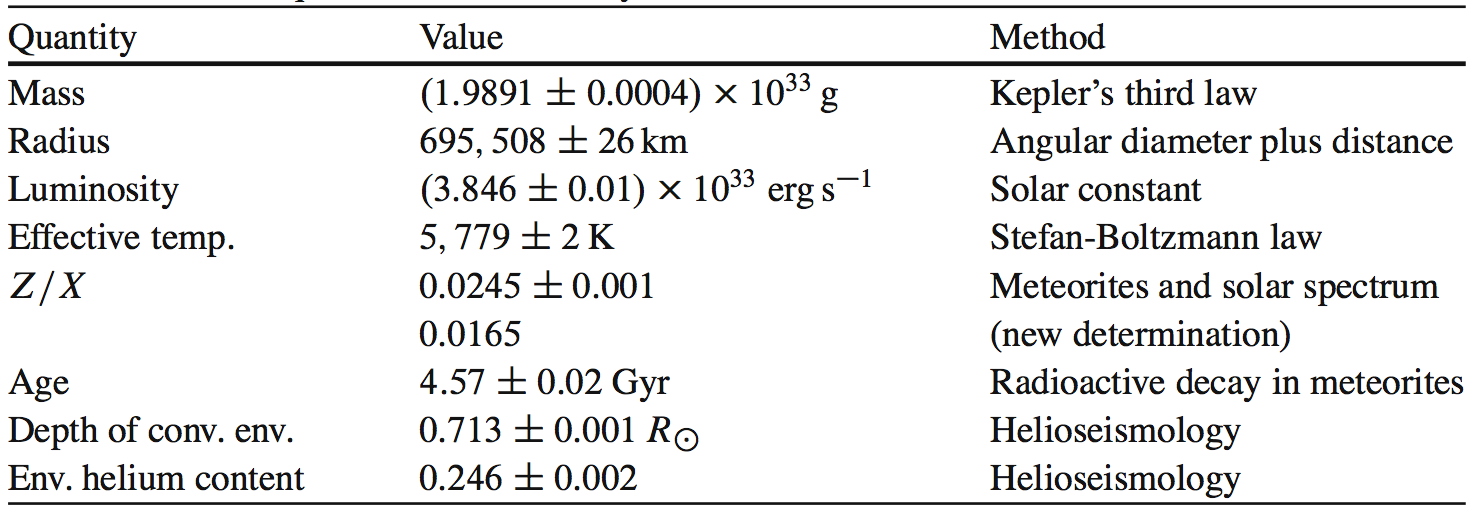
\includegraphics[width=14cm]{figures/SolarQuantities.png}
    \caption{\footnotesize{Solar quantities and how they are derived. Table taken from Kippenhahn, Weigert \& Weiss (2012).}}
    \label{table:solarquantities}
\end{table}

{\noindent}\textbf{Solar neutrinos:} Some of the nuclear reactions of the pp chain, as well as of the CNO cycle, produce neutrinos. In addition, there are also neutrinos due to the very rare \textit{pep} and \textit{hep} reactions

\begin{align*}
    {\rm ^1H+^1H+e^- \rightarrow ^2H+\nu\,(\textit{pep})} \\
    {\rm ^3He+^1H \rightarrow ^4He+e^++\nu\,(\textit{hep})},
\end{align*}

{\noindent}the latter one being the trivial way to produce $^4$He after the \textbf{pp-chain},

\begin{align*}
    {\rm ^1H+^1H \rightarrow ^2H+e^++\nu,} \\
    {\rm ^2H+^1H \rightarrow ^3He+\gamma},
\end{align*}

but it is occurring in only $10^{-8}$ of all cases. However, the energy of the emitted neutrino is close to $10\,{\rm MeV}$, and it is therefore necessary to consider this reaction. The neutrinos leave the star practically without interacting with the stellar matter. The energy spectrum of neutrinos from $\beta$ decay is continuous, since the electrons can take part of the energy away, while neutrinos released after an inverse $\beta$ decay are essentially monochromatic. Therefore most reactions of the pp chain have a continuous spectrum, while the pep-reaction and the electron capture on $^7$Be have a line spectrum. Since $^7$Be can decay into $^7$Li either in the ground state or in an excited state, this reaction gives two spectral lines. The neutrino spectrum of the Sun as predicted from the reactions of the pp chain, computed from our standard solar model, is given in Figure \ref{fig:neutrinospectrum}.

{\noindent}Since the solar neutrinos can leave the Sun almost unimpeded they can in principle be measured in terrestrial laboratories and thus be used to learn directly about conditions in the innermost solar core. This difficult task indeed has been undertaken since 1964, when John Bahcall and Raymond Davies began to plan for an underground neutrino detector in a mine in Homestead, North Dakota. Forty years later the experiments finally have confirmed the standard solar model, and R. Davies received the Nobel Prize for his work. The time in between, however, was characterized by the \textbf{solar neutrino problem}.

{\noindent}The solar neutrino problem consisted in the fact that since the first results from the so-called chlorine experiment by Davies there was a lack of neutrinos compared to solar model predictions. The chlorine experiment is sensitive to neutrinos with energies above $0.814\,{\rm MeV}$ and therefore, as can be seen in Figure \ref{fig:neutrinospectrum} mainly to the $^8$B neutrinos, with some contribution from pep, hep, and $^7$Be neutrinos. The experiment is based on the reaction $^{37}Cl+\nu\rightarrow^{37}Ar$, where the decays of radioactive argon nuclei are counted. The rate of neutrino captures is commonly measured in solar neutrino units (SNU). One SNU corresponds to $10^{-36}$ captures per second and per target nucleus. The predicted counts amount to $7.5\,{\rm SNU}$ for the chlorine experiment, the measurements averaged over several decades to only $2.5\pm0.2\,{\rm SNU}$. The deficit could indicate that the solar centre is cooler than in the models.

{\noindent}To improve the experimental evidence, additional experiments were started. First, another kind of radio-chemical detector using gallium in the detector fluid measured, due to a much lower energy threshold, the majority of neutrinos, including those from the pp-reaction. Later, electron-scattering detectors were developed, which are sensitive to the highest energies only, but which provide directional information about the neutrino source (for these detectors the \textit{hep}-neutrinos of have to be taken into account.). All experiments confirmed that the solar neutrino flux was of the right order of magnitude, and therefore that indeed the Sun shines by the nuclear fusion of hydrogen, but they also consistently measured a deficit of neutrinos. This deficit, however, varied between different kinds of detectors.

{\noindent}With more and more experimental data it became evident that even hypothetical changes to the solar centre cannot solve the problem and that the solution is most likely to be found in the properties of neutrinos. All nuclear reactions emit electron neutrinos, and these are the only ones that were measured in terrestrial experiment, with the exception of the electron-scattering Sudbury Neutrino Observatory (SNO) experiment in Canada, where heavy water (with a high percentage of deuterium isotopes) was used as the detector. Here also reactions with the two other types (flavours) of neutrinos, muon and tau neutrinos can be detected. Summing these and the electron neutrinos up, the total number of detections is completely consistent with the solar model prediction, within a few percent. What created the apparent solar neutrino deficit is the fact that neutrinos can change their flavour, both while travelling through vacuum and more efficiently in the presence of electrons in the solar interior. A similar effect was also confirmed for muon neutrinos arising in the Earth's upper atmosphere from high-energy cosmic radiation, when measured before or after they have travelled through the Earth's interior. The modelling of the solar interior, together with sophisticated experiments, has therefore resulted in new knowledge about fundamental properties of neutrinos. In particular, these so-called \textbf{neutrino oscillations} are possible only if neutrinos have mass.

\begin{figure}[t]
    \floatbox[{\capbeside\thisfloatsetup{capbesideposition={right,top},capbesidewidth=4cm}}]{figure}[\FBwidth]
    {\caption{\footnotesize{The neutrino spectrum of the Sun as predicted from the theoretical standard solar model. The solid lines belong to reactions of the pp chain while the broken lines are due to reactions of the CNO cycle. The neutrinos from most of the reactions have continuous spectra, while mono-energetic neutrinos come from $^7$Be and from the pep-reaction. The flux  for the continuum sources is given in $cm^2\,s^{-1}\,MeV^{-1}$ and for the line sources in $cm^2\,s^{-1}$. The sensitivity of the three types of neutrino experiments is indicated above the figure and by the shaded regions. Figure taken from Kippenhahn, Weigert \& Weiss (2012).}}
    \label{fig:neutrinospectrum}}
    {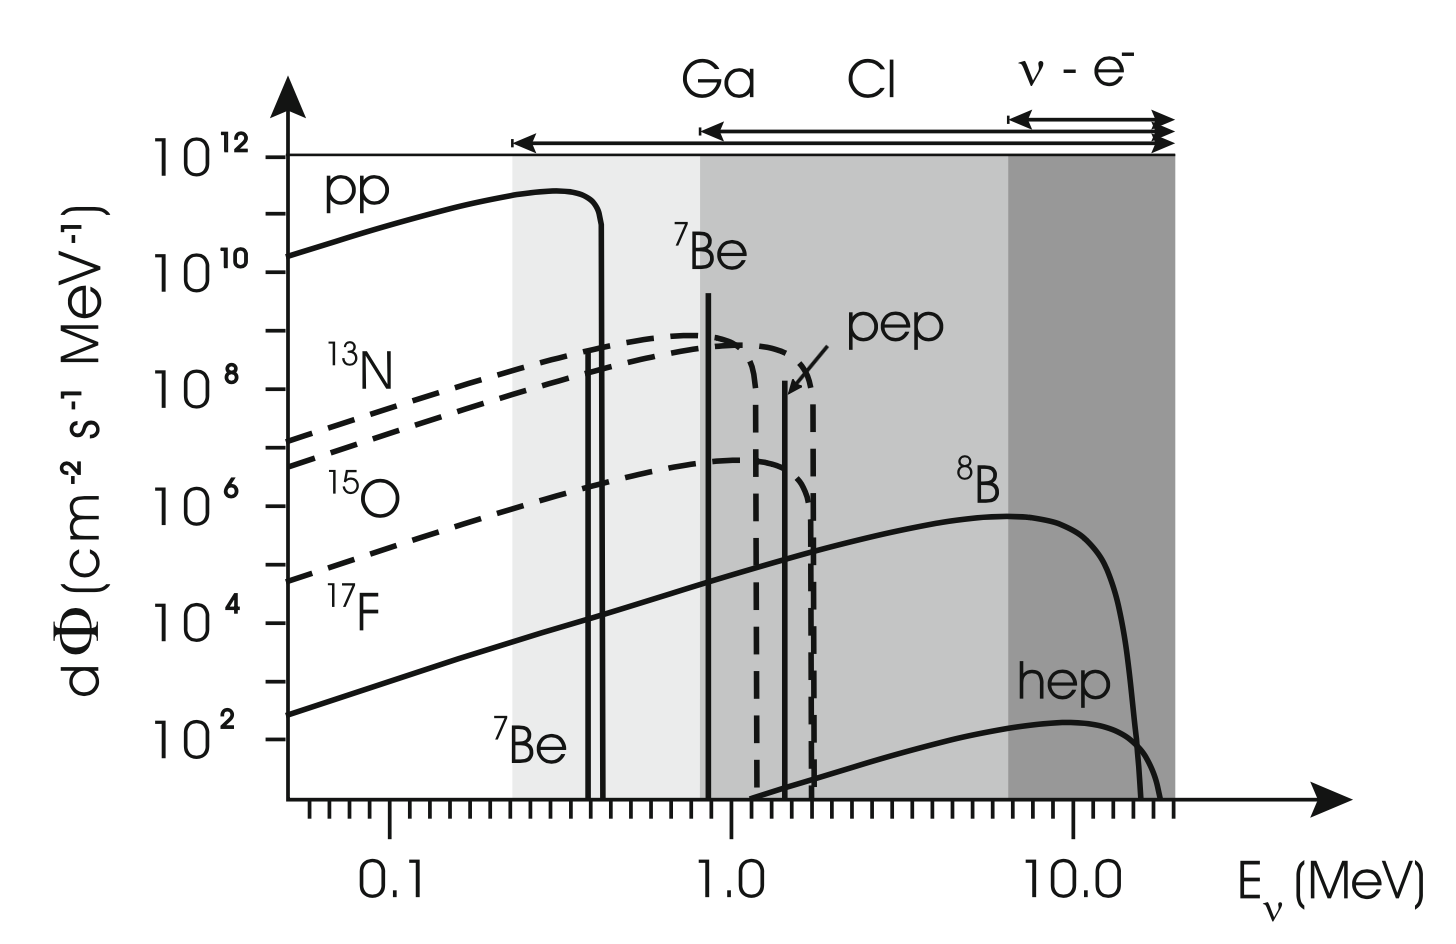
\includegraphics[width=10cm]{figures/NeutrinoSpectrum.png}}
\end{figure}

% --------------------------------------------------------------
%               11. 
% --------------------------------------------------------------

\newpage
\subsection{Question 11}

Which have higher central pressure, high-mass or low-mass main-sequence stars? Roughly, what is their mass-radius relation? Derive this.

\subsubsection{Short answer}

Answer.

\subsubsection{Additional context}

Additional context.
\subsubsection{Follow-up Questions}

\begin{itemize}
    \item How would we actually know the central pressure?
    \item What properties can we measure to test models of stellar structure?
\end{itemize}

% --------------------------------------------------------------
%               12. 
% --------------------------------------------------------------

\newpage
\subsection{Question 12}

Sketch the SED of an O, A, G, M, and T star. Give defining spectral characteristics, such as the Balmer lines and Balmer jump and Calcium doublets, and describe physically.

\subsubsection{Short answer}

Answer.

\subsubsection{Additional context}

Additional context.

\subsubsection{Follow-up Questions}

\begin{itemize}
    \item Are there emission lines?
    \item What molecular lines are in the Sun?
    \item What important lines are there are much longer wavelengths than those in the optical?
    \item What if the A star had a protoplanetary disk?
    \item What is the significance of a $\lambda$F$_\lambda$ (or $\nu$F$_\nu$) spectrum?
    \item How can the relative height of the stellar vs disk bumps change? (i.e., total energy of the system cannot change; dust bump can't be higher than star bump without extinction.)
\end{itemize}

% --------------------------------------------------------------
%               13. 
% --------------------------------------------------------------

\newpage
\subsection{Question 13}

What can be learned about young stars (T Tauri and pre-main-sequence stars) from an analysis of their spectral features?

\subsubsection{Short answer}

Answer.

\subsubsection{Additional context}

Additional context.

\subsubsection{Follow-up Questions}

\begin{itemize}
    \item How does the spectrum change as planets start to form?
\end{itemize}

% --------------------------------------------------------------
%               14. 
% --------------------------------------------------------------

\newpage
\subsection{Question 14}

Sketch the spectral energy distribution (SED) of a T Tauri star surrounded by a protoplanetary disk. How would the SED change: (a) if the disk develops a large inner hole, (b) if the dust grains in the disk grow in size by agglomeration (with the same total mass)?

\subsubsection{Short answer}

Answer.

\subsubsection{Additional context}

Additional context.

% --------------------------------------------------------------
%               15. 
% --------------------------------------------------------------

\newpage
\subsection{Question 15}

What are the primary origins of the heat lost to space by infrared luminosity of Jupiter, Earth, and Io?

\subsubsection{Short answer}

Answer.

\subsubsection{Additional context}

Additional context.

% --------------------------------------------------------------
%               16. 
% --------------------------------------------------------------

\newpage
\subsection{Question 16}

Explain the observational problem of radius inflation for hot Jupiters and describe two possible solutions.

\subsubsection{Short answer}

Answer.

\subsubsection{Additional context}

Additional context.

% --------------------------------------------------------------
%               17. 
% --------------------------------------------------------------

\newpage
\subsection{Question 17}

Explain the effects of an atmosphere on a planet’s surface temperature and the position of the “habitable zone”. What special considerations must one make for habitability around M-type stars?

\subsubsection{Short answer}

Answer.

\subsubsection{Additional context}

Additional context.

% --------------------------------------------------------------
%               18. 
% --------------------------------------------------------------

\newpage
\subsection{Question 18}

Explain the process of nuclear fusion and give two examples of important fusion processes that affect the lives of stars.

\subsubsection{Short answer}

Answer.

\subsubsection{Additional context}

Additional context.

% --------------------------------------------------------------
%               19. 
% --------------------------------------------------------------

\newpage
\subsection{Question 19}

What is Fermi’s Paradox? Explain its logic and assess the current state of the Paradox in light of modern knowledge.

\subsubsection{Short answer}

Answer.

\subsubsection{Additional context}

Additional context.

\subsubsection{Follow-up Questions}

\begin{itemize}
    \item What percentage of stars have planets?
\end{itemize}

% --------------------------------------------------------------
%               20. 
% --------------------------------------------------------------

\newpage
\subsection{Question 20}

The so-called r- and s- processes are mechanisms that produce elements heavier than iron. Describe these mechanisms and evidence for them from abundance patterns. Where is the r-process thought to act?

\subsubsection{Short answer}

Answer.

\subsubsection{Additional context}

Additional context.

% --------------------------------------------------------------
%               Resources 
% --------------------------------------------------------------

\newpage
\subsection{Resources}

\begin{itemize}
    \item Stellar Populations; Greggio \& Renzini (2011)
    \item The Fundamentals of Stellar Astrophysics, Collins (2003)
    \item Stellar Structure and Evolution, Kippenhahn, Weigert \& Weiss (2012)
    \item Evolution of Stars and Stellar Populations, Salaris \& Cassisi (2005)
    \item The Astronomical Reach of Fundamental Physics, Burrows \& Ostriker (2014)
    \item Opacity, Huebner \& Barfield (2014)
    \item Radiative Processes in Astrophysics, Rybicky \& Lightman (1979)
    \item Understanding Variable Stars, Percy (2007)
\end{itemize}

\end{document}
